\chapter{Divergent series}
\index{divergent series}
\label{2011-m-ch-ds}

\newthought{Power series approximations} often occur
in physical situations in the context of solutions of ordinary differential equations;
for instance in celestial mechanics or in quantum field theory.\cite{Boyd99thedevil,PhysRev.85.631}
According to Abel\cite{Hardy:1949} they
appear to be the ``invention of the devil,'' even more so as\cite{rousseau-2004}  {\em ``for the most part,
it is true that the results are correct, which is very strange.''}

There appears to be another, complementary, more optimistic and less perplexed, view on diverging series,
a view that has been expressed by Berry as follows:\cite{berry-92}
{\em ``$\ldots$ an asymptotic series $\ldots$ is a compact encoding of a function,
and its divergence should be regarded not as a deficiency but as a source of information about the function.''}
In a similar spirit, Boyd quotes {\em Carrier's Rule}:
{\em ``divergent series converge faster than convergent series because they don't have to converge.''}

\newthought{The intuition behind such statements} is based on the observation that,
while convergent series representing some function
may converge very slowly and numerically intractably,
\sidenote{Contemplate on the feasibility
of computing the partial sum $\sum_{j=0}^n \frac{(-1)^j x^{2j+1}}{(2j+1)!} =\sin_n (x)$
of the sine funtion without ``shortcuts;''
that is, without computing the remainder of $\frac{x}{2\pi}$, subject to some finite machine precision, say, for $x=10^5$.
Or consider the convergence of the general series solution of the $N$-body problem\cite{Diacu96}}
asymptotical divergent series
representations of functions
may yield reasonable estimates in ``low'' order before they diverge ``fast''
later on (for higher polynomial order).
Ritt's theorem
\index{Ritt's theorem}
\index{theorem of Ritt}
mentioned in Section~\ref{2019-mm-ch-ca-Ritt}
provides a formal basis for this conjecture.

\section{Convergence, asymptotic divergence, and divergence: A zoo perspective}

Let us first define {\em convergence} in the context of series.
\index{convergence}
\index{convergent series}
A series
\begin{equation}
s=\sum_{j=0}^\infty a_j =a_0+a_1+a_2+\cdots
\end{equation}
is said to converge to the {\em sum}
$s$ if the {\em partial sum}
\begin{equation}
s_n\equiv s(n)=  \sum_{j=0}^n a_j =a_0+a_1+a_2+\cdots + a_n
\end{equation}
tends to a finite limit $s$ when $n\rightarrow \infty$;
otherwise it is said to diverge (it may remain finite but may alternate).

A power series about some number $c\in \mathbb{C}$
depends on some additional parameter $z$; it has partial sums of the form
\begin{equation}
s_n (z)\equiv s(n,z) =
\sum_{j=0}^n a_j (z - c)^j =a_0+a_1 (z-c) +a_2(z-c)^2+\cdots + a_n (z-c)^n.
\end{equation}
If $c=0$ then the partial sum of this series  $s_n (z) =  \sum_{j=0}^n a_j z^j$
is about the origin.
Power series are important because they are used for solving ordinary differential equations,
such as Frobenius series \index{Frobenius series} in the theory of
differential equations of the Fuchsian type.
\index{Fuchsian equation}

Power series have a rich enough structure to leave room
for some ``grey area'' in-between divergence and convergence.
\index{asymptotic series}
\index{semi-convergent series}
\index{convergently beginning series}
In Dingle's terms,\cite{Dingle-1973}
{\em
``the designation `asymptotic series' will be reserved
for those series in which for large values of the variable at all phases
the terms first progressively decrease in magnitude, then reach a minimum
and thereafter increase.''}
Those series could be useful in the case of irregular singularities
of an ordinary differential equation, for which the Frobenius method fails.
We shall come back to asymptotic series later in Section~\ref{2019-mm-ch-ds-aps}.


% https://www.coursera.org/learn/advanced-calculus/lecture/koIrf/does-the-series-1-1-2-1-3-converge-or-diverge
For a start consider a widely known diverging series: the
{\em harmonic series}
\index{harmonic series}
\begin{equation}
s=  \sum_{j=1}^\infty \frac{1}{j} = 1+\frac{1}{2}+\frac{1}{3}+\frac{1}{4}+\cdots .
\end{equation}
A medieval proof by Oresme (cf. p.~92 of Ref.\cite[10mm]{Edwards-1979})
uses approximations: Oresme points out that increasing numbers of summands in the series can be rearranged to yield numbers bigger than, say, $\frac{1}{2}$;
more explicitly,
$\frac{1}{3}+\frac{1}{4}> \frac{1}{4}+\frac{1}{4}  =\frac{1}{2}$,
$\frac{1}{5}+ \cdots +\frac{1}{8} > 4 \frac{1}{8}  =\frac{1}{2}$,
$\frac{1}{9}+ \cdots +\frac{1}{16} > 8 \frac{1}{16}  =\frac{1}{2}$,
and so on, such that the entire series must grow larger as $\frac{n}{2}$.
As $n$ approaches infinity, the series is unbounded and thus diverges.




One of the most prominent divergent series is Grandi's series,\cite{Sloane_oeis.org/A033999}
sometimes also referred to as
\index{Grandi's series}
\index{Leibniz's series}
Leibniz series\cite{leibnitz-1860,moore-1938,Hardy:1949,everest-2003}
\begin{equation}
s = \sum_{j=0}^\infty (-1)^j=
\lim_{n \rightarrow \infty} \left[\frac{1}{2}+\frac{1}{2}\left( -1\right)^n\right]
=1-1+1-1+1-\cdots ,
\label{2009-fiftyfifty-1s}
\end{equation}
whose summands may be -- inconsistently
-- ``rearranged,''
yielding
\begin{equation*}
\begin{split}
\textrm{ either }
1-1+1-1+1-1+\cdots = (1-1)+(1-1)+(1-1)-\cdots =0\\
\textrm{ or }
1-1+1-1+1-1+\cdots = 1+(-1+1)+ (-1+1) +\cdots =1.
\end{split}
\end{equation*}
One could tentatively associate the arithmetical average $1/2$ to represent ``the sum of Grandi's series.''

Another tentative approach  would be to first regularize this nonconverging expression by introducing a ``small entity''
$\varepsilon$ with $0 < \varepsilon <1$, such that $\vert \varepsilon - 1 \vert  <1$, which allows to formally sum up the geometric series
\begin{equation*}
s_\varepsilon \stackrel{\text{def}}{=} \sum_{j=0}^\infty (\varepsilon -1)^j=\frac{1}{1-(\varepsilon -1)}   =\frac{1}{2- \varepsilon  };
\end{equation*}
and then take the limit $s \stackrel{\text{def}}{=}  \lim_{\varepsilon \rightarrow 0^+} s_\varepsilon
= \lim_{\varepsilon \rightarrow 0^+}  1/(2- \varepsilon  ) =   1/2$.

Indeed, by {\em Riemann's rearrangement theorem},
\index{Riemann rearrangement theorem}
convergent series  which do not absolutely converge
(i.e., $\sum_{j=0}^n a_j$ converges but $\sum_{j=0}^n \left| a_j \right|$ diverges)
may be brought to  ``converge'' to arbitrary (even infinite) values
by permuting (rearranging) the (ratio of) positive and negative terms
(the series of which must both be divergent).

These manipulations
\marginnote{Every such strategy involving {\em finite means} fails miserably.}
could be perceived in terms of certain
paradoxes of infinity, such as Hilbert's hotel
\index{Hilbert's hotel}
which always has vacancies -- by ``shifting all of its guests one room further
down its infinite corridor''.\cite{rucker}



\section{Geometric series}
\index{geometric series}

As Grandi's series is a particular, ``pathologic,'' case of a {\em geometric series}
\index{geometric series}
we shall briefly review those in greater generality.
A finite geometric (power) series is defined by
(for convenience a multiplicative constant is ommitted)
\begin{equation}
\begin{split}
s_n(z)\equiv s(n,z) =
\sum_{j=0}^n z^j
=\underbrace{z^0}_{1}+z+z^2+  \cdots + z^n
.
\end{split}
\label{2019-mm-ch-ds-fgs}
\end{equation}
Multiplying both sides of
(\ref{2019-mm-ch-ds-fgs})
by $z$ gives
\begin{equation}
\begin{split}
z s_n(z)
= \sum_{j=0}^n z^{j+1}
=z+z^2+z^3+  \cdots + z^{n+1}
.
\end{split}
\label{2019-mm-ch-ds-fgsmbr}
\end{equation}
Subtracting
(\ref{2019-mm-ch-ds-fgsmbr})
from the original series
(\ref{2019-mm-ch-ds-fgs})
yields
\begin{equation}
\begin{split}
s_n(z) - z s_n(z)
= (1 - z)s_n(z)
= \sum_{j=0}^n z^{j} - \sum_{j=0}^n z^{j+1} \\
=
1+z+z^2+  \cdots + z^n
-
\left(z+z^2+z^3+  \cdots + z^{n+1}\right)
=1-z^{n+1},
\end{split}
\label{2019-mm-ch-ds-fgsmbrs}
\end{equation}
and
\begin{equation}
s_n(z)=  \frac{1-z^{n+1}}{1 - z}.
\label{2019-mm-ch-ds-fgsmbrss}
\end{equation}
Alternatively, by defining a ``remainder'' term
\begin{equation}
r_n(z)\stackrel{\text{def}}{=} \frac{z^{n+1}}{z-1},
\label{2019-fiftyfifty-1sgs-remainder}
\end{equation}
(\ref{2019-mm-ch-ds-fgsmbrss})
can be recasted into
\begin{equation}
\begin{split}
\frac{1}{1 - z}= s_n(z)+  \frac{z^{n+1}}{1 - z} = s_n(z) - r_n(z)\text{; and} \\
s_n(z) = \frac{1}{1-z} + r_n(z) = \frac{1}{z - 1} + \frac{z^{n+1}}{z-1}
.
\end{split}
\label{2019-mm-ch-ds-fgsmbrss1}
\end{equation}
\marginnote{Again the symbol ``$O$'' stands for ``of the order of'' or ``absolutely bound by'' in the following way:
if $g(x)$ is a positive function,  then $f(x)=O\left(g(x)\right)$
implies that there exist a positive real number $m$
such that $\vert f(x) \vert < m g(x)$. }.
\index{order of}
\index{big $O$ notation}
\index{Bachmann-Landau notation}
\index{asymptotic notation}
As $z \rightarrow 1$  the remainder diverges because the denominator tends to zero.
As $z \rightarrow -1$, again  the remainder diverges; but for a different reason: it does not converge
to a unique limit but alternates between $\pm \frac{1}{2}$.
If $\vert z\vert > 1$  the remainder  $r_n(z) = \frac{z^{n+1}}{1 - z} =O( z^n )$
grows without bounds; and
therefore the entire sum (\ref{2019-mm-ch-ds-fgs}) diverges in the $n\rightarrow \infty$ limit.


Only for $\vert z\vert <1$
the remainder  $r_n(z) = \frac{z^{n+1}}{1 - z} =O( z^n )$
vanishes in the $n\rightarrow \infty$ limit;
and, therefore, the infinite sum in the geometric series exists and
converges as a limit of~(\ref{2019-mm-ch-ds-fgs}):
\begin{equation}
\begin{split}
s(z) =
\lim_{n\rightarrow \infty}
s_n(z)=
\lim_{n\rightarrow \infty}
\sum_{j=0}^n z^j
=  z^j=1+z+z^2+  \cdots     \\
=1+ z(1+z+  \cdots)  =1+z s(z).
\end{split}
\label{2009-fiftyfifty-1sgs}
\end{equation}
Since $s(z)=1+z s(z)$
and
$s(z)-z s(z)=s(z)(1-z)=1$,
\begin{equation}
s(z)= \sum_{j=0}^\infty z^j= \frac{1}{1-z}.
\label{2012-fiftyfifty-1sgscont}
\end{equation}



\section{Abel summation  -- assessing paradoxes of infinity}
\index{Abel sum}

One ``Abelian'' way to ``sum up'' divergent series is by ``illegitimately continuing''
the argument
%of a finite geometric series   (\ref{2019-mm-ch-ds-fgs})
to  values for which the
infinite geometric series diverges;
thereby only taking its ``finite part''~(\ref{2012-fiftyfifty-1sgscont})
while at the same time neglecting or disregarding
the divergent remainder term~(\ref{2019-fiftyfifty-1sgs-remainder}).


For Grandi's series
this essentially amounts to substituting $z= - 1$
into~(\ref{2012-fiftyfifty-1sgscont}), thereby defining the
{\em Abel sum} (denoted by an ``A'' on top of equality sign)
\index{Abel sum}
\begin{equation}
s=\sum_{j=0}^\infty(-1)^j  = 1-1+1-1+1-1+\cdots \stackrel{{\rm A}}{=} \frac{1}{1-(-1)} = \frac{1}{2}.
\label{2012-fiftyfifty-1sgscont1}
\end{equation}



Another ``convergent value of a divergent series''
can, by a similar transgression of common syntatic rules,
be ``obtained'' by ``formally  expanding''  the square of the Abel sum of
Grandi's series
$
s^2 \stackrel{{\rm A}}{=} [1-(-x)]^{-2} = (1+x)^{-2}
$ for  $x=1$
into the Taylor series\cite{Kline-83}
around $t=0$, and using   $(-1)^{j-1}=(-1)^{j-1}(-1)^{2}=(-1)^{j+1}$:
\begin{equation}
\begin{split}
s^2   \stackrel{{\rm A}}{=} (1+x)^{-2}  \Big|_{x =1}=
\left.\left\{\left.\sum_{j=0}^\infty \frac{1}{j!}\left[\frac{d^j}{d{t}^j}  (1+t)^{-2}\right]   (x-t)^j\right|_{t=0}\right\} \right|_{x=1}
\\
=
\sum_{j=0}^\infty (-1)^j (j+1) =
\sum_{j=0}^\infty (-1)^{j+1} k =
1-2+3-4+5-\cdots
.
\label{2009-fiftyfifty-1s1}
\end{split}
\end{equation}
On the other hand, squaring the Grandi's series ``yields'' the Abel sum
\index{Grandi's series}
\begin{equation}
s^2 =
\left(\sum_{j=0}^\infty (-1)^j\right)
\left(\sum_{k=0}^\infty (-1)^k\right)
\stackrel{{\rm A}}{=} \left(\frac{1}{2}\right)^2=\frac{1}{4},
\end{equation}
so that, one could ``infer'' the Abel sum
\begin{equation}
s^2 =
1-2+3-4+5-\cdots  \stackrel{{\rm A}}{=} \frac{1}{4}.
\end{equation}


Once this identification is established, all of Abel's hell breaks loose:
One could, for instance, ``compute the finite sum\cite{Sloane_oeis.org/A000217} of all natural numbers\cite{Sloane_oeis.org/A000027}''
(a sum even mentioned on page~22 in a book on String Theory\cite{polchinski_1998}),
{\it via} formal analytic continuation as for the
Ramanujan summation~(\ref{2019-mm-ch-ds-Ramanujan}):  \index{Ramanujan summation}
\begin{equation}
S  =
\sum_{j=0}^\infty j = 1+2+3+4+5 + \cdots
\stackrel{{\rm A}}{=} \lim_{n\rightarrow \infty} \frac{n(n+1)}{2}
\stackrel{{\rm A}}{=} - \frac{1}{12}
\label{2016-m-ch-ds-natnumser}
\end{equation}
by sorting out
\begin{equation}
\begin{split}
S - \frac{1}{4}\stackrel{{\rm A}}{=}
S-s^2  = 1+2+3+4+5 + \cdots -
(1-2+3-4+5-\cdots )   \\
= 4 + 8+ 12 +  \cdots = 4 S
,
\label{2016-m-ch-ds-natnumser2}
\end{split}
\end{equation}
so that  $3 S
\stackrel{{\rm A}}{=}  - \frac{1}{4}$,
and, finally, $S
\stackrel{{\rm A}}{=}  - \frac{1}{12}$.

Note that the sequence of the partial sums $s^2_n=\sum_{j=0}^n (-1)^{j+1} j $
of $s^2$, as expanded in (\ref{2009-fiftyfifty-1s1}),
``appears to yield'' every integer once; that is,
$s^2_0 =0$,
$s^2_1 =0+1=1$,
$s^2_2 =0+1-2=-1$,
$s^2_3 =0+1-2+3=2$,
$s^2_4 =0+1-2+3-4=-2$,
$\ldots$,
$s^2_n =-\frac{n}{2}$ for even $n$,
and
$s^2_n =-\frac{n+1}{2}$ for odd $n$.
It thus establishes a strict one-to-one mapping
$s^2: {\Bbb N} \mapsto {\Bbb Z}$
of the natural numbers onto the integers.

These ``Abel sum'' type manipulations are outside of the radius of convergence
of the series and therefore cannot be expected to
result in any meaningful statement.
They could, in a strict sense, not even be perceived in terms of certain
paradoxes of infinity, such as Hilbert's hotel.
If they could quantify some sort of ``averaging'' remains questionable.
One could thus rightly consider any such
exploitations of infinities
as not only meaningless but outrightly wrong
-- even more so when committing to transgressions of convergence criteria.
Note nevertheless, that great minds have contemplated
geometric series for ever-decreasing ``Zeno squeezed'' computation cycle times,\cite[-30mm]{Russell-36,weyl:49}
or wondered in which state a (Thomson) lamp \index{Thomson lamp}   would
be after an infinite number of switching cycles
whose ever-decreasing switching times allow a geometric progression.\cite{thom:54}

\section{Riemann zeta function and Ramanujan  summation: Taming the beast}
\label{2019-mm-ds-zetafr}
\index{Ramanujan summation}


Can we make any sense\marginnote{For proofs and additional information see \S~3.7 in  \bibentry{Tao-2013}.}  of the seemingly absurd statement of the last section -- that
an infinite sum of all (positive) natural numbers appears to be both negative and ``small;'' that is, $-\frac{1}{12}$?
In order to set things up
let us introduce a generalization of the harmonic series:
the Riemann zeta function (sometimes also referred to as the Euler-Riemann zeta function)
\index{zeta function}
\index{Riemann zeta function}
\index{Euler-Riemann zeta function}
defined for $\Re t > 1$ by
\begin{equation}
\zeta (t) \stackrel{{\rm def}}{=}
\sum_{j=1}^\infty \frac{1}{j^t}
=
\prod_{p\;{\rm prime}} \left(\sum_{j=1}^\infty p^{-jt}\right)
=
\prod_{p\;{\rm prime}} \frac{1}{1-\frac{1}{p^t}}
\label{2016-m-ds-zeta}
\end{equation}
can be  continued analytically to all complex values $t\neq 1$.
Formally this analytic continuation yields the following
{\em Ramanujan summations}  (denoted by an ``R'' on top of equality sign)
for $t=0,-1,-2$ as follows\sidenote{For $t=-1$ this  has been ``derived''  earlier.}:
\begin{equation}
\begin{split}
1+1+1+1+1 + \cdots = \sum_{j=1}^\infty 1 \stackrel{R}{=} \zeta (0)  = -\frac{1}{2}
, \\
1+2+3+4+5 + \cdots = \sum_{j=1}^\infty j \stackrel{R}{=}  \zeta (-1)  = -\frac{1}{12}
, \\
1+4+9+16+25 + \cdots = \sum_{j=1}^\infty j^2 \stackrel{R}{=}  \zeta (-2)  = 0;
\end{split}
\label{2019-mm-ch-ds-Ramanujan}
\end{equation}
or, more generally,
for $s=1,2,\ldots$,
%  https://terrytao.wordpress.com/2010/04/10/the-euler-maclaurin-formula-bernoulli-numbers-the-zeta-function-and-real-variable-analytic-continuation
\begin{equation}
1+2^s+3^s+4^s+5^s + \cdots = \sum_{j=1}^\infty j^s \stackrel{R}{=} \zeta (-s) = -\frac{B_{s+1}}{ s+1}
,
\end{equation}
where $B_s$ are the
{\em Bernoulli numbers}.\cite{Sloane_oeis.org/A027642}
\index{Bernoulli numbers}

This scheme can be extended\cite{Masina-Grandi} to ``alternated''
zeta functions
\begin{equation}
1-2^s+3^s-4^s+5^s - \cdots =\sum_{j=1}^\infty \frac{(-1)^{j+1}}{j^s}
=      - \sum_{j=1}^\infty \frac{(-1)^j}{j^s} %\stackrel{R}{=}  \eta (s)
\end{equation}
by subtracting a similar series containing all even summands
twice:
\begin{equation}
\begin{split}
\sum_{j=1}^\infty \frac{(-1)^{j+1}}{j^s}
=
-\sum_{j=1}^\infty \frac{(-1)^j}{j^s}
=
\sum_{j=1}^\infty \frac{ 1 }{j^s}
-
2 \sum_{j=1}^\infty \frac{ 1 }{ (2j)^s}
%= \sum_{j=1}^\infty \frac{ 1 }{j^s} - 2 \sum_{j=1}^\infty \frac{ 1 }{(2^t)(j^s)}
\\
\stackrel{R}{=}
\zeta (s) - \frac{2}{2^s}\zeta (s)
%=  \left(1  - \frac{1}{2^{s-1}}\right)  \zeta (s)
=
\left(1  -2^{1-s} \right)   \zeta (s)
=\eta (s).
\end{split}
\label{2019-mm-ch-ds-Ramanujan-eta}
\end{equation}
$\eta (t) = \left(1  -2^{1-t} \right)   \zeta (t)  $
stands for the {\em Dirichlet eta function}.
\index{Dirichlet eta function}

By~(\ref{2019-mm-ch-ds-Ramanujan-eta}),  like in the Abel case, Grandi's series
corresponds to $s=0$, and sums up to
\begin{equation}
\begin{split}
1-1+1- \cdots = \sum_{j=1}^\infty \frac{(-1)^{j+1}}{j^0}  \stackrel{R}{=} \eta (0)  =  \left(1  - 2^1\right)  \zeta (0)
= -\zeta (0) = \frac{1}{2}
.
\end{split}
\label{2019-mm-ch-ds-Ramanujan-eta-Grandi}
\end{equation}

One way mathematicians cope with ``difficult entities''
such as generalized functions or divergent series is
to introduce suitable ``cutoffs'' in the form of multiplicative functions
and work with the resulting ``truncated'' objects instead.
We have encountered this both in Ritt's theorem
\index{Ritt's theorem}
\index{theorem of Ritt}
(cf. Section~\ref{2019-mm-ch-ca-Ritt}
on page~\pageref{2019-mm-ch-ca-Ritt})
and by inserting test functions associated with distributions
(cf. Chapter~\ref{2011-m-ch:gf}).

Therefore,
as Tao has pointed out,
if the divergent sums are multiplied with suitable ``smoothing'' functions\sidenote{An example of such smoothing function is
$\eta (x) = \theta\left(x^2-1\right) \exp \left(\frac{x^2}{x^2-1}\right)$, and, therefore,
$\eta \left(\frac{x}{N}\right) = \theta\left(x^2-N^2\right) \exp \left( \frac{x^2}{x^2-N^2}\right)$
defined in~(\ref{2019-m-ch-di-tf1-mod1})
on page~\pageref{2019-m-ch-di-tf1-mod1}.}
$\eta \left(\frac{j}{N}\right)$  which are
bounded, have a compact support,
and tend to $1$ at $0$ -- that is, $\eta (0) = 1$ for ``large $N$'' --
the respective smooth summations yield  smoothed asymptotics.
Then the divergent series
can be (somehow superficially\cite{Candelpergher-2017}) ``identified with''  their respective constant terms of their smoothed partial
sum asymptotics.

More explicitly, for the sum of natural numbers, and, more generally, for any fixed $s\in \mathbb{N}$ this yields\cite{Tao-2013}
\begin{equation}
\begin{split}
\sum_{j=1}^\infty j \eta \left(\frac{j}{N}\right)
= - \frac{1}{12} + C_{\eta ,1} N^2 + O\left(\frac{1}{N}\right)
,  \\
\sum_{j=1}^\infty j^s \eta \left(\frac{j}{N}\right)
= - \frac{B_{s+1}}{s+1} + C_{\eta ,s} N^{s+1} + O\left(\frac{1}{N}\right)
,
\end{split}
\label{2019-mm-ch-ds-Ramanujan-snn}
\end{equation}
where   $C_{\eta ,s}$ is the
{\em Archimedean factor}
\index{Archimedean factor}
\begin{equation}
\begin{split}
C_{\eta ,s}
\stackrel{\text{def}}{=}
\int_0^\infty x^s \eta (x) dx
.
\end{split}
\label{2019-mm-ch-ds-Ramanujan-af}
\end{equation}
Observe that~(\ref{2019-mm-ch-ds-Ramanujan-snn})
forces the Archimedean factor $C_{\eta ,1}$ to be positive and ``compensate for'' the constant factor
$-\frac{B_{s+1}}{s+1}$, which, for $s=1$, is negative and $-\frac{B_{2}}{2}=-\left(\frac{1}{6}\right)\left(\frac{1}{2}\right)=-\frac{1}{12}$.
In this case, as $N$ gets large, the sum diverges with $O\left(N^2\right)$, as can be expected from Gauss' summation formula $1+2+...+N= \frac{N(N+1)}{2}$
for the  the partial sum of the natural numbers up to $N$.

As can be expected both sides of (\ref{2019-mm-ch-ds-Ramanujan-snn}) diverge in the limit $N \rightarrow \infty$ and thus
$\eta \left(\frac{j}{N}\right)\rightarrow \eta (0)=1$.
For $s=1$ this could be interpreted as an instance of Ritt's theorem;
for arbitrary $s\in \mathbb{N}$ as a generalization thereof.


\section{Asymptotic power series}
\label{2019-mm-ch-ds-aps}


Divergent (power) series appear to be
living in the ``grey area'' in-between convergence and divergence, and, if
treated carefully,
may still turn out to be useful; in particular, when it comes to numerical approximations:
the first few terms of divergent series may (but not always do) ``converge''
to some ``useful functional'' value.
Alas, by taking into account more and more terms,
these series expansions eventually ``degrade'' through the rapidly increasing additional terms.
These cases have been termed asymptotic,\cite[-90mm]{Erdelyi-1956,Bender-Orszag,Balser-1994} semi-convergent, or convergently beginning series.
Asymptoticity has already been defined
in Section~\ref{2019-mm-ch-ca-Ritt} (on page~\pageref{2019-mm-ch-ca-Ritt}).
\index{asymptoticity}

Thereby the pragmatic emphasis is on a proper and ``useful'' (versus disadvantageous) {\em representation}
or {\em encoding} of entities such as functions and solutions of
ordinary differential equations by power series -- differential equations
with irregular singular points which are
not of the Fuchsian type, and not solvable by the Frobenius method.

The heuristic (not exact)
\index{optimal truncation rule}%\cite{Boyd99thedevil}
{\em optimal truncation rule}
\sidenote{This pragmatic approach may cause some ``digestion problems;''
see Heaviside's remarks on page~\pageref{2013-m-ch-intro-cooking}.}
suggests that the best approximation to a function value from its divergent asymptotic
series expansion is often obtained by truncating the series (before or) at its smallest term.


{
\color{blue}
\bexample


To get a feeling for what can be expected in such scenarios
consider a ``canonical'' example:
With regard to convergence
the Stieltjes function\cite{Bleistein-Handelsman}
(formula~5.1.28, page~230 of Abramowitz and Stegun\cite[0mm]{abramowitz:1964:hmf} but with $x \mapsto \frac{1}{x}$)
\index{Stieltjes function}
\begin{equation}
\begin{split}
S(x)   = \int_0^\infty    \frac{e^{-t}}{1+tx} dt  = \frac{1}{x}  \int_0^\infty    \frac{e^{-t}}{\frac{1}{x}+t} dt
\end{split}
\label{2019-m-ch-ds-Stieltjes-function}
\end{equation}
can be represented by
power and inverse factorial series in three different ways:
\marginnote{In a metamatematical interpretation one might perceive mathematical entities such as functions
as ``ontologically'' existing in a ``Platonist universe of ideas''.
However, ontologic ``existence'' need not necessarily entail
concrete, operational, algorithmic ``epistemic access'' by formalizable means necessary for, say, physical prediction.
Therefore, pragmatic access to these functions presents an epistemic issue depending on our respective capacities and means to do so;
that is, it becomes means relative.}
\begin{itemize}
\item[(i)]
by the asymptotic Stieltjes series: for $n \in \mathbb{N}$,
\index{Stieltjes series}
\begin{equation}
\begin{split}
S(x) =
   \underbrace{\sum_{j=0}^n (-x)^j j!  }_{=S_n(x)}
+  \underbrace{(-x)^{n+1}(n+1)! \int_0^\infty   \frac{e^{-t}}{(1+tx)^{n+2}} dt}_{=R_n(x)},
\end{split}
\label{2019-m-ch-ds-asymptotic-Stieltjes-series}
\end{equation}
\item[(ii)]
by convergent Maclaurin series such as (Ramanujan found a series which converges even more rapidly)
\begin{equation}
\begin{split}
S(x)
=  \frac{e^\frac{1}{x}}{x}  \Gamma \left( 0, \frac{1}{x} \right)
=  -\frac{e^\frac{1}{x}}{x}  \left[  \gamma - \log x +\sum_{j=1}^\infty \frac{(-1)^j}{j!j x^j} \right]
,
\end{split}
\label{2019-m-ch-ds-Stieltjes-series}
\end{equation}
where

\begin{equation}
\gamma
=\lim_{n\rightarrow \infty}\left(
\sum_{j=1}^n \frac{1}{j}- \log n
\right) \approx 0.5772
\end{equation}
is the Euler-Mascheroni constant.\cite[-10mm]{Sloane_oeis.org/A001620}
\index{Euler-Mascheroni constant}
$\Gamma (z,x)$ represents the upper incomplete gamma function defined in~(\ref{2017-m-ch-sf-edgamma}).
\index{incomplete gamma function}

\item[(iii)]
by an inverse factorial series~\cite{Weniger2010}
\begin{equation}
S(x)= \sum_{j=0}^\infty \frac{(-1)^j}{\left(\frac{1}{x}\right)_{j+1}} \sum_{k=0}^j {S}_j^{(k)} k!,
\label{2022-afssf}
\end{equation}
where
$\left(x\right)_{j}=\Gamma \left(x+j\right)/\Gamma \left( x \right) = x \left(x +1\right)\cdots \left( x + j - 1 \right)$
and $(x)_0=1$
are Pochhammer symbols~(\ref{2011-m-ch-sfsf}) introduced on page~\pageref{2011-m-ch-sfsf},
\index{Pochhammer symbol}
and ${S}_j^{(k)}$
are Sterling numbers of the first kind
\index{Sterling numbers of the first kind}
that are the polynomial coefficients of the
Pochhammer symbol $(z-j+1)_j$
(Section~24.1.3, page~824 of Abramowitz and Stegun\cite[-15mm]{abramowitz:1964:hmf});
that is [cf. Equation(\ref{2022-m-ch-dsifps})],
\begin{equation}
\sum_{k=0}^j {S}_j^{(k)} z^k
= (z-j+1)_j
%= (z-j+1) (z+1-j+1)   \cdots (z+1) z
= (-1)^j  (-z)_j
\label{2022-ch-snfk}
\end{equation}
for $j \in \mathbb{N}\cup \{0\}$.
%\marginnote{
$(-1)^{j-k}{S}_j^{(k)}>0$
can also be identified with the (positive) number of permutations of $n$ symbols which have exactly $m$ cycles.
Because of the factor $(-1)^{j-k}$, as $j$ is fixed and $k$ varies, ${S}_j^{(k)}$ are strongly oscillating.
%}
We conjecture without proof that in the inner sum of~(\ref{2022-afssf})
there are ``substantial'' cancellations.
The general method of conversion of a power series into an inverse factorial series will be discussed in the next section~\ref{2022-factser}.
\end{itemize}

A complete derivation\cite[-5mm]{sommer-Stieltjes}
of the Maclaurin series~(ii) is omitted; we just note that
the Stieltjes function $S(x)$ for real positive $x>0$ can be rewritten in terms of
the exponential integral
\index{exponential integral}
%which is, for the phase [argument; cf.~Equation~(\ref{2012-m-ch-ca-ef})]
%\index{argument}
%\index{phase}
%$\vert \varphi \varphi < \pi$ of $z=re^{i\varphi}$,  defined by
(e.g., formul\ae~5.1.1, 5.1.2, 5.1.4, page~227 of Abramowitz and Stegun\cite{abramowitz:1964:hmf})
\marginnote{See also \url{http://mathworld.wolfram.com/En-Function.html},
\url{http://functions.wolfram.com/GammaBetaErf/ExpIntegralEi/introductions/ExpIntegrals/ShowAll.html}
as well as  \bibentry{Masina-EIntegral}.}
\begin{equation}
\begin{split}
E_1(y) =   -\text{Ei}(-y)
= \Gamma \left( 0, y \right)
=
\int_{1}^\infty    \frac{e^{-uy}}{u} du
=
\int_{y}^\infty    \frac{e^{-u}}{u} du
\end{split}
\label{2019-m-ch-ds-Stieltjes-Ei}
\end{equation}
% http://mathworld.wolfram.com/En-Function.html
% https://en.wikipedia.org/wiki/Exponential_integral
by first substituting $x=\frac{1}{y}$ in $S(x)$ as defined in~(\ref{2019-m-ch-ds-Stieltjes-function}), followed by the transformation of integration variable
$t = y(u-1)$, so that, for $y>0$,
\begin{equation}
\begin{split}
S\left(\frac{1}{y}\right)
=  \int_0^\infty    \frac{e^{-t}}{1+\frac{t}{y}} dt\\
[\text{substitution } t = y(u-1)\text{, }u=1+\frac{t}{y}\text{, }dt =y du]\\
=  \int_1^\infty    \frac{e^{-y(u-1)}}{1+\frac{y(u-1)}{y}} y du\\
=ye^{y}\int_1^\infty    \frac{e^{-yu}}{u}  du
=  ye^{y}E_1(y)  =  -ye^{y}\text{Ei}(-y)
\text{, or}\\
S(x)=  \frac{e^\frac{1}{x}}{x} E_1\left(\frac{1}{x}\right)
%=  -\frac{e^\frac{1}{x}}{x}\text{Ei}\left(-\frac{1}{x}\right)
= \frac{e^\frac{1}{x}}{x} \Gamma \left( 0, \frac{1}{x} \right)
.
\end{split}
\label{2019-m-ch-ds-Stieltjes-function-Ei}
\end{equation}
The asymptotic Stieltjes
series~(\ref{2019-m-ch-ds-asymptotic-Stieltjes-series})
quoted in (i)
as well as the convergent
series~(\ref{2019-m-ch-ds-Stieltjes-series})
quoted in (ii)
can, for positive (real) arguments, be obtained by substituting the respective series for the exponential integral
(e.g., formul\ae~5.1.51, page~231 and~5.1.10,5.1.11, page~229  of Abramowitz and Stegun):
%\marginnote{see also http://mathworld.wolfram.com/En-Function.html}
% FullSimplify[ -EulerGamma - Log[y] - Sum[((-1)^j y^j)/(j! j ), {j, 1, Infinity}]]
\begin{equation}
\begin{split}
E_1(y)
\sim
\frac{e^{-y}}{y}\sum_{j=0}^\infty (-1)^j j!  \frac{1}{y^j} =
\frac{e^{-y}}{y} \left( 1 - \frac{1}{y}  + 2 \frac{1}{y^2} + 6 \frac{1}{y^3} + \cdots
\right) \\
 = \Gamma \left( 0, y \right)=- \gamma - \log y - \sum_{j=1}^\infty \frac{ (-y)^j }{j (j!)}
,
\end{split}
\label{2019-m-ch-ds-Stieltjes-Ei-se}
\end{equation}
where again $\gamma$ stands for the Euler-Mascheroni constant
and $\Gamma (z,x)$ represents the upper incomplete gamma function
(cf. Formula~6.5.1, p~260   of Abramowitz and Stegun)
defined in~(\ref{2017-m-ch-sf-edgamma}).
\marginnote{It would be wrong but tempting
-- and would make the estimation of the remainder easier --
to treat the divergent series
very much like a geometric series outside its radius of convergence.}


The
divergent remainder of the asymptotic Stieltjes
series~(\ref{2019-m-ch-ds-asymptotic-Stieltjes-series})
can be estimated
by successive partial integrations of the Stieltjes function
and induction:
\begin{equation}
\begin{split}
S(x) =  \int_0^\infty    \frac{e^{-t}}{1+tx} dt
=
-\left. \frac{e^{-t}}{1+tx}\right \vert_{t=0}^{t=\infty}
-
x \int_0^\infty    \frac{xe^{-t}}{(1+tx)^2} dt  \\
= 1-      x \int_0^\infty    \frac{e^{-t}}{(1+tx)^2} dt\\
= 1-  x+    2x^2 \int_0^\infty    \frac{e^{-t}}{(1+tx)^2} dt\\
= 1-  x+    2x^2 \int_0^\infty    \frac{e^{-t}}{(1+tx)^3} dt\\
= 1-  x+    2x^2 -6 x^3\int_0^\infty    \frac{e^{-t}}{(1+tx)^4} dt\\
\vdots  \\
=\underbrace{\sum_{j=0}^n (-x)^j j!  }_{=S_n(x)}
+  \underbrace{(-x)^{n+1}(n+1)!   \int_0^\infty   \frac{e^{-t}}{(1+tx)^{n+2}} dt}_{=R_n(x)}
.
\end{split}
\label{2019-m-ch-ds-Stieltjes-function-pi}
\end{equation}
%
%
%
%
\begin{marginfigure}
{\color{black}
\begin{center}
\begin{tabular}{c}
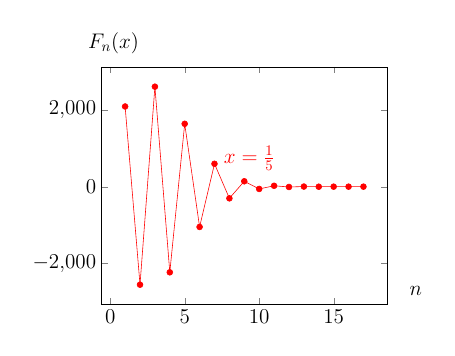
\begin{tikzpicture} [ scale=0.53, every mark/.append style={mark size=2pt} ]
\begin{axis}[ %ymode=log,
    %log ticks with fixed point,
    ticklabel style = {font=\Large },
    %ymax=1,
    x label style={font=\Large ,at={(axis description cs:1.1,0.1)}},
    y label style={font=\Large ,at={(axis description cs:0.15,1.1)},rotate=270},
    xlabel={$n$},
    ylabel={$F_n(x)$},
    yticklabel style={
        /pgf/number format/fixed,
        /pgf/number format/precision=5
                     },
    scaled y ticks=false
]

\addplot  [
red, mark=*
]  table {   %  x = 1/5; Print[  Grid[Table[{n,    N[(E^(1/x)/x) (-EulerGamma - Log[1/x] -  Sum[(-1)^j /(j! j  x^j), {j, 1, n}]) - (E^(1/x)/x) Gamma[0, 1/x]]}, {n, 1, 30}]]]
1       2086.84
2       -2551.08
3       2602.16
4       -2229.
5       1635.93
6       -1048.05
7       595.202
8       -303.45
9       140.329
10      -59.3718
11      23.1491
12      -8.3693
13      2.82067
14      -0.890289
15      0.264232
16      -0.0740067
17      0.0196234
}
node [pos=0.9,label={[xshift=1.0cm, yshift=0.3cm, style={font=\Large}]$x=\frac{1}{5}$} ]{};

\end{axis}
\end{tikzpicture}
\\
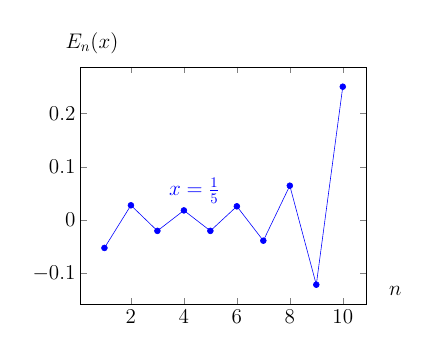
\begin{tikzpicture} [ scale=0.53, every mark/.append style={mark size=2pt} ]
\begin{axis}[ %ymode=log,
    %log ticks with fixed point,
    ticklabel style = {font=\Large },
    %ymax=1,
    x label style={font=\Large ,at={(axis description cs:1.1,0.1)}},
    y label style={font=\Large ,at={(axis description cs:0.15,1.1)},rotate=270},
    xlabel={$n$},
    ylabel={$E_n(x)$},
    yticklabel style={
        /pgf/number format/fixed,
        /pgf/number format/precision=5
                     },
    scaled y ticks=false
]
\addplot  [
blue, mark=*
]  table {   % x = 1/5; Print[Grid[  Table[{n, N[ Sum[(-1)^j j! x^j, {j, 0, n}] - (E^(1/x)/x) Gamma[0, 1/x]]}, {n, 1, 30}]]]
1       -0.0521109
2       0.0278891
3       -0.0201109
4       0.0182891
5       -0.0201109
6       0.0259691
7       -0.0385429
8       0.0646763
9       -0.121118
10      0.250471
}
node [pos=0.2,label={[xshift=1.0cm, yshift=0.3cm, style={font=\Large}]$x=\frac{1}{5}$} ]{};

\end{axis}
\end{tikzpicture}
\\
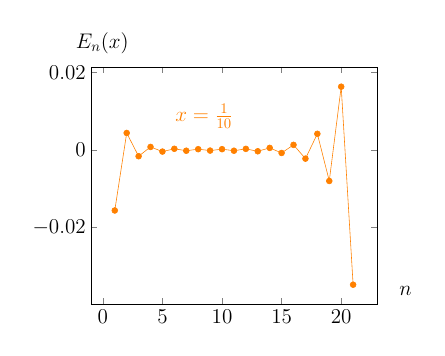
\begin{tikzpicture} [ scale=0.53, every mark/.append style={mark size=2pt} ]
\begin{axis}[ %ymode=log,
    %log ticks with fixed point,
    ticklabel style = {font=\Large },
    %ymax=1,
    x label style={font=\Large ,at={(axis description cs:1.1,0.1)}},
    y label style={font=\Large ,at={(axis description cs:0.15,1.1)},rotate=270},
    xlabel={$n$},
    ylabel={$E_n(x)$},
    yticklabel style={
        /pgf/number format/fixed,
        /pgf/number format/precision=5
                     },
    scaled y ticks=false
]
\addplot  [
orange, mark=*
]  table {   % x = 1/10; Print[Grid[  Table[{n, N[ Sum[(-1)^j j! x^j, {j, 0, n}] - (E^(1/x)/x) Gamma[0, 1/x]]}, {n, 1, 30}]]]
1       -0.0156333
2       0.00436666
3       -0.00163334
4       0.000766661
5       -0.000433339
6       0.000286661
7       -0.000217339
8       0.000185861
9       -0.000177019
10      0.000185861
11      -0.000213307
12      0.000265694
13      -0.000357008
14      0.000514775
15      -0.000792899
16      0.00129938
17      -0.00225749
18      0.00414488
19      -0.00801963
20      0.0163094
21      -0.0347816
}
node [pos=0.2,label={[xshift=1.0cm, yshift=0.3cm, style={font=\Large}]$x=\frac{1}{10}$} ]{};

\end{axis}
\end{tikzpicture}
 \\
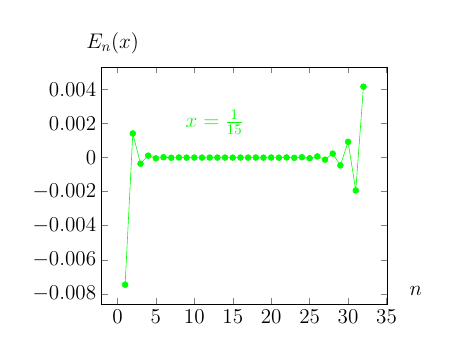
\begin{tikzpicture} [ scale=0.53, every mark/.append style={mark size=2pt} ]
\begin{axis}[ %ymode=log,
    %log ticks with fixed point,
    ticklabel style = {font=\Large },
    %ymax=1,
    x label style={font=\Large ,at={(axis description cs:1.1,0.1)}},
    y label style={font=\Large ,at={(axis description cs:0.15,1.1)},rotate=270},
    xlabel={$n$},
    ylabel={$E_n(x)$},
    yticklabel style={
        /pgf/number format/fixed,
        /pgf/number format/precision=5
                     },
    scaled y ticks=false
]
\addplot  [
green, mark=*
]  table {   % x = 1/15; Print[  Grid[Table[{n,   AccountingForm[ N[Sum[(-1)^j j! x^j, {j, 0, n}] - (E^(1/x)/x) Gamma[0, 1/x]], 20, NumberSigns -> {"-", "+"}]}, {n, 1, 40}]]]
1       -0.0074708532778055
2       +0.001418035611083335
3       -0.0003597421666944323
4       +0.0001143319073796389
5       -0.00004369278397831078
6       +0.00001951709256486911
7       -0.00000998084982195557
8       +0.000005751386117691659
9       -0.000003687955446141089
10      +0.000002604938929784417
11      -0.000002009850279205416
12      +0.000001681981087964246
13      -0.000001517606096901325
14      +0.00000146867527561767
15      -0.000001517606096901325
16      +0.000001667760700430065
17      -0.000001942321669945457
18      +0.000002389777174482965
19      -0.00000309754802829687
20      +0.000004218885575557607
21      -0.000006024121470105115
22      +0.00000899895553019281
23      -0.00001403642920350112
24      +0.00002282018637023153
25      -0.0000386075062525082
26      +0.00006786716096018885
27      -0.0001237872400228213
28      +0.0002339676418122716
29      -0.0004576917964023153
30      +0.000925627080027081
31      -0.001933231931260382
32      +0.004165667292819641
}
node [pos=0.2,label={[xshift=1.0cm, yshift=0.3cm, style={font=\Large}]$x=\frac{1}{15}$} ]{};

\end{axis}
\end{tikzpicture}
\end{tabular}
\end{center}
\caption{The series approximation error   $F_n(x)= -\frac{e^\frac{1}{x}}{x}  \left[  \gamma - \log x +\sum_{j=1}^n \frac{(-1)^j}{j!j x^j} \right] -S(x)$
of the convergent Stieltjes series~(\ref{2019-m-ch-ds-Stieltjes-series})
for $x=\frac{1}{5}$, and
$E_n(x)=S_n(x) -S(x)$
of the Stieltjes series~(\ref{2019-m-ch-ds-asymptotic-Stieltjes-series})  as a function of increasing $n$
for $x\in \left\{ \frac{1}{5},\frac{1}{10},\frac{1}{15}\right\}$.}
  \label{2018-mm-ferrorS}
}
\end{marginfigure}
%
%
%
%
For $x>0$ the absolute value of the remainder $R_n(x)$
can be estimated to be bound from above by
\begin{equation}
\begin{split}
\vert R_n(x)\vert
=(n+1)! \, x^{n+1} \int_0^\infty   \frac{e^{-t}}{(1+xt)^{n+2}} dt
\le (n+1)! \, x^{n+1} \underbrace{\int_0^1    e^{-t} dt}_{=1}.
%=(n+1)! \, x^{n+1} \int_0^\infty   \frac{e^{-t}}{(1+xt)^{n+2}} dt \\
%\ge (n+1)! \, x^{n+1} \int_0^1   \frac{e^{-t}}{(1+x)^{n+2}} dt \\
%= (n+1)!
% \underbrace{\frac{x^{n+1}}{(1+x)^{n+2}}}_{O\left(\frac{1}{x}\right)}
%\underbrace{\int_0^1    e^{-t} dt}_{= O(1)} \\
%=  (n+1)! O\left(\frac{1}{x}\right)
\end{split}
\label{2019-m-ch-ds-Stieltjes-function-pi-re}
\end{equation}
By examining\cite[9mm]{Erdelyi-1956} the partial series $\left| S_n(x) \right|=  \sum_{j=0}^n j! x^j$
with   the bound on the remainder $\left| R_n(x) \right| \le (n+1)!  \, x^{n+1}$
it can be inferred that  the bound on the remainder is of the same magnitude as the
first ``neglected''  term $(n+1)! x^{n+1}$.

A comparison of the argument $x$ of the Stieltjes series
with the number $n$ of terms contributing to $S_n(x)$ reveals three regions:
\begin{itemize}
\item[(i)] if $x=0$ the remainder vanishes for all $n$ and the series converges towards the constant $1$ (regardless of $n$).
\item[(ii)] if $x>1$ the series diverges; no matter what (but could be subjected to ``resummation procedures'' {\it \`a la} Borel,
cf Sections~\ref{2019-mm-ds-bresum}{\&}\ref{2019-mm-ch-ds-rsdg});
\item[(iii)] if $x = 1/y<1$ (and thus $y>1$)  the remainder $
\left| R_n\left(\frac{1}{y}\right) \right| \le \frac{(n+1)!}{y^{n+1}}   )$  is dominated by the $y$ term
until about $n=y$; at which point the factorial takes over and
the partial sum
$S_n(x)$ starts to become an increasingly worse approximation.


Therefore, although the
Stieltjes series is divergent for all $x>0$, in the domain $0<x<1$
it behaves very much like a convergent series until
about $n \approx x < 1$. In this $0< x < 1$ regime it makes sense to define an error estimate $E_k(x)=S_n(x)-S(x)$
as the difference between the partial sum $S_n(x)$, taken at $x$ and including terms up to the order of $x^n$,
and the exact value $S(x)$.

Figure~\ref{2018-mm-ferrorS}
depicts the asymptotic divergence of $S_n(x)$ for
$x\in \{\frac{1}{5},\frac{1}{10},\frac{1}{15}\}$
up to the respective adapted values $n \approx \frac{1}{x}$.
Since in the kernerls of the sums of the asymptotic Stieltjes series~(\ref{2019-m-ch-ds-asymptotic-Stieltjes-series})
$k_j(x)= (-1)^j j! x^j $
and the convergent Stieltjes series~(\ref{2019-m-ch-ds-Stieltjes-series})
$\frac{(-1)^j}{j!j x^j} = \frac{\left[k_j(x)\right]^{-1}}{ j }$
are ``almost inverse''   it can be expected that, for $0<x<1$, and if one is only willing to take ``the first view'' terms of these respective sums,  then the
former asymptotic Stieltjes series~(\ref{2019-m-ch-ds-asymptotic-Stieltjes-series}) will perform better than the latter
convergent Stieltjes series~(\ref{2019-m-ch-ds-Stieltjes-series})
the smaller $x\ll 1$   is.


\end{itemize}

 \eexample
 }

\section{Conversion of power series into inverse factorial series}
\index{factorial series}
\label{2022-factser}

\marginnote{The following recasting of power series into inverse factorial series closely follows \bibentry{Weniger2010}.}

We have already encountered a conversion of power series into inverse factorial series when discussing one ``epistemic access'' to, that is,
one representation of, the Stieltjes function in Equation~\ref{2022-afssf}.
In what follows  general power series
$f(z) = \sum_{n=0}^\infty a_n z^n$ will be rewritten
into (inverse) factorial series~\cite[-90mm]{Watson1912,Doetsch1972}
\begin{equation}
\begin{split}
f(z)
=
\alpha_0 \frac{1}{z}
+
\alpha_1 \frac{1!}{z(z+1)}
+
\alpha_2 \frac{2!}{z(z+1)(z+2)}+
\ldots
= \sum_{n=0}^\infty \alpha_n \frac{n!}{(z)_{n+1}}
,
\end{split}
\label{2022-m-ch-dsfs}
\end{equation}
where $(z)_{n+1}$ are Pochhammer symbols
\index{Pochhammer symbol}
which have been introduced in Equation~(\ref{2011-m-ch-sfsf}).
Thereby the main ``ingredient'' will be Sterling numbers
\index{Sterling numbers of the first kind}
which are defined and reviewed in Section~24.1.3, page~824 of Abramowitz and Stegun\cite[-20mm]{abramowitz:1964:hmf}.


To accomplish this task we first rewrite the power series in $z$ into an inverse power series in $\frac{1}{z}$
\begin{equation}
\begin{split}
f(z)
= \sum_{n=0}^\infty a_n z^n
= \frac{1}{z}  \sum_{n=0}^\infty \frac{a_n}{\left(\frac{1}{z}\right)^{n+1}}
.
\end{split}
\label{2022-m-ch-dsinv}
\end{equation}

\marginnote{Cf. Equation~(6), \S~30, p.~78 in  \bibentry{Nielsen-Gammafunktion}, as well as Equation~(A.14) in  \bibentry{Weniger2010}.}
Stirling numbers of the first kind~(\ref{2022-ch-snfk})
\index{Stirling numbers of the first kind}
${S}_j^{(n)}$
have infinite generating functions.
These serve as ``translations''---that is, as expansions from
an (inverse) power $\frac{1}{z^{n+1}}$ in terms of  inverse  factorial series $(z)_{n+j+1}$:
for $k  \in \mathbb{N} \cup \{0\}$,
\begin{equation}
\begin{split}
\frac{1}{z^{n+1}}  = \sum_{j=0}^\infty \frac{(-1)^j}{(z)_{n+j+1}} {S}_{n+j}^{(n)}
.
\end{split}
\label{2022-m-ch-dsngf}
\end{equation}
$(z)_{k+j+1}$ are Pochhammer symbols
\index{Pochhammer symbol}
introduced in Equation~(\ref{2011-m-ch-sfsf}).

The respective ``reverse'' expansion of a Pochhammer symbol $(z)_{k+1}$ in terms of  an inverse power series
$\frac{1}{z^{n+j+1}}$
for $k  \in \mathbb{N} \cup \{0\}$ and $\vert z \vert >0$
is given by
\begin{equation}
\begin{split}
\frac{1}{(z)_{n+1}}  = \sum_{j=0}^\infty \frac{(-1)^j}{z^{n+j+1}} {S}_{n+j}^{(n)}
.
\end{split}
\label{2022-m-ch-dsngfinverse}
\end{equation}
\marginnote{Cf. Equation~(9), \S~26, ~p.~68 in  \bibentry{Nielsen-Gammafunktion}, as well as Equation~(A.11) in  \bibentry{Weniger2010}.}



Insertion of~(\ref{2022-m-ch-dsngf})  into~(\ref{2022-m-ch-dsinv}), rearranging the order of the summations through an index shift $m = n+j$ yields
\begin{equation}
\begin{split}
f(z)
= \frac{1}{z}  \sum_{n=0}^\infty a_n \sum_{j=0}^\infty \frac{(-1)^j}{\left(\frac{1}{z}\right)_{n+j+1}} {S}_{n+j}^{(n)}
\\
= \frac{1}{z}  \sum_{j=0}^\infty \sum_{n=0}^\infty a_n \;  \frac{(-1)^j}{\left(\frac{1}{z}\right)_{n+j+1}} {S}_{n+j}^{(n)}
\\
[[ m = n+j \text{ with }  n \ge 0 \text{ and }  j \ge 0
\\
\Rightarrow  m \ge 0  \text{ and } j = m - n \ge 0 \Rightarrow m \ge n \text{ or }  n \le m]]
\\
= \frac{1}{z} \sum_{m=0}^\infty   \frac{(-1)^m}{\left(\frac{1}{z}\right)_{m+1}} \sum_{n=0}^m (-1)^{\pm n} \; {S}_{m}^{(n)} \; a_n
.
\end{split}
\label{2022-m-ch-dsinv2}
\end{equation}
So if we define the inverse power series
\begin{equation}
\begin{split}
f'(u)
= z f(z)
= \frac{1}{u} f\left( \frac{1}{u} \right)
= \sum_{m=0}^\infty \frac{a'_m}{u^{m+1}}
= \sum_{m=0}^\infty b_m' \, \frac{m!}{(u)_{m+1}}
,
\end{split}
\label{2022-m-ch-comp1}
\end{equation}
with $u=1/z$,
then, by comparison,
%$c_m = (-1)^m \sum_{n=0}^m (-1)^n \; a_n \; {S}_{m}^{(n)}$.
%Because ${S}_{0}^{(0)}=1$ taking only the first term $m=0$ in~(\ref{2022-m-ch-dsinv2}) results in  $f(z)= a_0$.
\begin{equation}
\begin{split}
b_m'= \frac{1}{m!} \frac{1}{\left(u \right)_{m+1}} \sum_{n=0}^m \underbrace{(-1)^{m\pm n}  \; {S}_{m}^{(n)}}_{>0} \; a_n'
.
\end{split}
\label{2022-m-ch-comp}
\end{equation}

{\color{OliveGreen}
\bproof

In what follows we turn to the proof of the Stieltjes factorial series~(\ref{2022-afssf}) in terms of the  Stirling's factorial series.
Stirling's factorial series,
\index{Stirling's factorial series}
also known as Waring's formula,
\index{Waring's formula}
can be derived by iteration for $\Re (z - w) > 0$
\marginnote{For a derivation of Stirling's factorial series see \S~30,~p.~77 in  \bibentry{Nielsen-Gammafunktion}.}\begin{equation}
\begin{split}
\frac{1}{z} \sum_{j=0}^\infty \left( \frac{w}{z} \right)^j=
\frac{1}{z}\cdot \frac{1}{1-\frac{w}{z}}  \\
=\frac{1}{z-w} =
\frac{1}{z} + \frac{w}{z(z-w)}=
\sum_{n=0}^\infty  \frac{(w)_n}{(z)_{n+1}}
,
\end{split}
\label{2022-m-ch-dswaring}
\end{equation}
where $\Re z$ stands for the real part of $z$.
\index{Pochhammer symbol}
$(w)_n$ and $(z)_{n+1}$ are Pochhammer symbols.

Note that $(z-n+1)_n$ in~(\ref{2022-ch-snfk}) can be rewritten as  $(-1)^j  (-z)_j$
since the following identity for Pochhammer symbols hold:
\begin{equation}
\begin{split}
(a-n+1)_n = \underbrace{(a-n+1)(a+1-n+1) \cdots (a-1)a}_{n\text{ times}} \\
= (-1)^n (-a+n-1)(-a-1+n-1) \cdots (-a+1)(-a)  \\
= (-1)^n  (-a)(-a+1) \cdots (-a-1+n-1)(-a+n-1) \\
= (-1)^n  (-a)_n
.
\end{split}
\label{2022-m-ch-dsifps}
\end{equation}
By replacing $z$ by $-z$ in  $(z-n+1)_n=(-1)^n  (-z)_n$  we obtain from
Equation~(\ref{2022-ch-snfk})---that is, from
$(z-j+1)_j = \sum_{k=0}^j z^k  {S}_j^{(k)}$,
\begin{equation}
\begin{split}
(z-n+1)_n = (-1)^n  (-z)_n  = \sum_{k=0}^n z^k  {S}_n^{(k)},
\\
(-z)_n  = (-1)^n  \sum_{k=0}^n z^k  {S}_n^{(k)}
,
\\
[[\text{or, with } z \mapsto -z, ]]
\\
(z)_n = (-1)^n  \sum_{k=0}^n (-1)^k  z^k {S}_n^{(k)}
.
\end{split}
\label{2022-m-ch-dsifps22}
\end{equation}

Insertion of~(\ref{2022-m-ch-dswaring})
with $w = -t$ and~(\ref{2022-m-ch-dsifps22})
with $-z = -t$
into~(\ref{2019-m-ch-ds-Stieltjes-function}), that is, into $S(x)   =  \frac{1}{x}  \int_0^\infty    \frac{e^{-t}}{\frac{1}{x}+t} dt$, yields~(\ref{2022-afssf}):
\begin{equation}
\begin{split}
S(z)
= \frac{1}{z}  \int_0^\infty    \frac{e^{-t}}{\frac{1}{z}+t} dt
= \frac{1}{z}  \int_0^\infty  \sum_{n=0}^\infty  \frac{(-t)_n}{\left(\frac{1}{z}\right )_{n+1}} e^{-t} dt
\\
= \frac{1}{z}  \sum_{n=0}^\infty  \frac{(-1)^n }{\left(\frac{1}{z}\right )_{n+1}}   \sum_{k=0}^n  {S}_n^{(k)} \underbrace{\int_0^\infty  t^k  \, e^{-t} dt}_{=\Gamma(k+1)=k!}
\\
=\frac{1}{z} \sum_{n=0}^\infty \frac{(-1)^n}{\left(\frac{1}{z}\right)_{n+1}} \sum_{k=0}^n {S}_n^{(k)} k!
.
\end{split}
\label{2022-m-ch-dsafssf}
\end{equation}

\bproof
}

\marginnote{For a discussion of convergence see  Section~3 of \bibentry{Weniger2010}, as well as \bibentry{Nielsen-Gammafunktion}, and \bibentry{landau1906uber}.}
Let us briefly consider the convergence of the
the  inverse factorial series (\ref{2022-m-ch-dsfs}), that is, of
$\sum_{n=0}^\infty  a_n \,{n!}/{(z)_{n+1}}= \sum_{n=0}^\infty  a_n \, {n!}/{\left[\Gamma(z+n+1)/\Gamma(z)\right]}$.
Note that its terms of the form $a_n {n!}/{(z)_{n+1}}$
can be estimated by considering the factor  ${n!}/{(z)_{n+1}}$, and with the help of
$\Gamma(z+a)/\Gamma(z+b)= z^{a-b}\left[1 + O\left(\frac{1}{z}\right) \right]$ for $z\rightarrow \infty$
({\S}~6, Formula~6.1.47  on p.~257  of Abramowitz and Stegun),%\cite[10mm]{abramowitz:1964:hmf}),
as follows:
\begin{equation}
\begin{split}
\frac{n!}{(z)_{n+1}}
= \frac{\Gamma(n+1)}{\left[\Gamma(z+n+1)/\Gamma(z)\right]}
= \frac{\Gamma(n+1)}{\Gamma(n+1+z)} \Gamma(z)  \\
= (n+1)^{-z}\left[1 + O\left(\frac{1}{n+1}\right) \right](z-1)!
= O \left( n^{-z} \right) \text{ for } n \rightarrow \infty.
\end{split}
\label{2022-m-ch-estimate}
\end{equation}

Therefore, the  inverse factorial series (\ref{2022-m-ch-dsfs})
converges with the possible
exception of the points $z =-m$ with $m \in   \mathbb{N} \cup \{0\}$
(where the Pochhammer symbols in the denominator might vanish)
if and only if the associated Dirichlet series
\index{Dirichlet series}
$\sum_{n=1}^\infty a_n \, n^{-z}$
converges.

A Dirichlet series has an abscissa of convergence
\index{abscissa of convergence}
$\Re (z) > \lambda$, that is, it converges on this half-plane.
$\lambda =- \infty$ in which case the Dirichlet series converges uniformly, or
$\lambda = \infty$ in which case the Dirichlet series diverges uniformly.
\marginnote{For a discussion of the convergence of Dirichlet series, see for instance \S~58,~255, page~456 of   \bibentry{Knoop1996}.}
Even if the inverse power series diverges factorially the respective inverse factorial series may converge; but this has to be
checked explicitly.

However, a convergence issue encountered in inverse factorial series is the Stokes phenomenon~\cite{Costin2016Aug,Costin_2017}:
the asymptotic behavior of functions need not be uniform in different regions of the complex plane, bounded by (anti-)Stokes lines.
In particular, inverse factorial series may not be suitable for the study of Stokes phenomena if Stokes lines
are present in the right complex half-plane $\Re ( \alpha ) > \lambda $ because of the singularities on these Stokes lines.
One may conjecture that inverse factorials might converge in regions where the associated power series are Borel summable;
yet convergence fails in the presence of Stokes lines.
This would mean that quantum field theories have convergent inverse factorial expansions only in less than four dimensions.

\section{Borel's resummation method -- ``the master forbids it''}
\index{Borel resummation}
\label{2019-mm-ds-bresum}

In what follows we shall review
%\cite[-20mm]{rousseau-2004}
a resummation method
%\sidenote[][-50mm]{For more resummation techniques, please see
%Chapter 16 of
%http://users.physik.fu-berlin.de/~kleinert/b8/psfiles/16.pdf }
invented by Borel\cite[-13mm]{Borel1899}
\marginnote{{\em ``The idea that a function could be determined by a divergent asymptotic series was a foreign one to the nineteenth century mind.
Borel, then an unknown young man, discovered that his summation method gave the ``right'' answer for many classical divergent series.
He decided to make a pilgrimage to Stockholm to see Mittag-Leffler, who was the recognized lord of complex analysis.
Mittag-Leffler listened politely to what Borel had to say and then,
 placing his hand upon the complete works by Weierstrass, his teacher, he said in Latin,
``The Master forbids it.''} quoted as {\em A tale of Mark Kac} on page 38  by  \bibentry{reed-sim4}.}
to obtain the exact convergent solution
(\ref{2011-m-ch-dseefasol})
of the differential equation  (\ref{2011-m-ch-dsee})
from the divergent series solution (\ref{2011-m-ch-dseess}).
First note that a suitable infinite series  can be rewritten as an integral,
thereby using the integral representation
(\ref{2011-m-ch-sfgamman}\&\ref{2017-m-ch-sf-edgamma})
$
n! = \Gamma ( n+1 ) =
\int_0^\infty t^{n}e^{-t}dt
$
% and (\ref{2011-m-ch-dsee15})
of the factorial
as follows:
\begin{equation}
\begin{split}
\sum_{j=0}^\infty
a_j
=
\sum_{j=0}^\infty
a_j  \frac{j!}{j!}
=
\sum_{j=0}^\infty
  \frac{a_j}{j!}  j!
\\
=
\sum_{j=0}^\infty
  \frac{a_j}{j!}  \int_0^\infty t^j e^{-t} dt
\stackrel{{\rm B}}{=}
\int_0^\infty \left(\sum_{j=0}^\infty   \frac{a_j t^j}{j!}\right)   e^{-t} dt
.
\end{split}
\label{2012-m-ch-dsborel}
\end{equation}



A series  $\sum_{j=0}^\infty   a_j $
is {\em Borel summable}
\index{Borel summable}
if
$\sum_{j=0}^\infty   \frac{a_j t^j}{j!}$ has a non-zero radius of convergence,
if it can be extended along the positive real axis, and if the integral
(\ref{2012-m-ch-dsborel}) is convergent.
This integral is called the
{\em Borel sum}
\index{Borel sum}
of the series.
It can be obtained by taking $a_j$, computing the sum $\sigma (t) = \sum_{j=0}^\infty   \frac{a_j t^j}{j!}$,
and integrating $\sigma (t)$ along the positive real axis with a ``weight factor'' $e^{-t}$.


More generally, suppose
\begin{equation}
S(z)= z \sum_{j=0}^\infty
a_j  z^j  = \sum_{j=0}^\infty
a_j  z^{j+1}
\label{2018-m-ch-ds-fps}
\end{equation}
is some formal power series.
Then  its {\em Borel transformation}
\index{Borel transformation}
is defined by
\begin{equation}
\begin{split}
\sum_{j=0}^\infty
a_j z^{j+1}
=
\sum_{j=0}^\infty
a_j z^{j+1}  \frac{j!}{j!}
=
\sum_{j=0}^\infty
  \frac{a_j z^{j+1} }{j!}  \underbrace{j!}_{ \int_0^\infty t^j e^{-t}   dt }  \\
=
\sum_{j=0}^\infty
  \frac{a_jz^{j} }{j!}  \int_0^\infty t^j e^{-t} z dt
\stackrel{{\rm B}}{=}
\int_0^\infty \left(\sum_{j=0}^\infty   \frac{a_j (z t)^j}{j!}\right)  e^{-t} z dt \\
[\textrm{variable substitution }  y= z t, \; t = \frac{y}{z}  , \; dy = z \,dt, \; dt = \frac{dy}{z}]\\
\stackrel{{\rm B}}{=}
\int_0^\infty \left(\sum_{j=0}^\infty   \frac{a_j y^j}{j!}\right)  e^{-\frac{y}{z}}   dy  =
\int_0^\infty {\cal B}S (y)  e^{-\frac{y}{z}}   dy
.
\end{split}
\label{2012-m-ch-dsboreltrafo}
\end{equation}

Often, this is written with $z=1/t$, such that the  Borel transformation
\index{Borel transformation}
is defined by
\begin{equation}
\begin{split}
\sum_{j=0}^\infty
a_j t^{-(j+1)}
\stackrel{{\rm B}}{=}
\int_0^\infty {\cal B}S (y)  e^{- yt }   dy
.
\end{split}
\label{2012-m-ch-dsboreltrafo2}
\end{equation}


The {\em Borel transform}\sidenote[][0mm]{This definition differs from the standard definition of the Borel
transform  based on coefficients $a_j$ with $S(z)=   \sum_{j=0}^\infty
a_j  z^{j}$ introduced in
 \bibentry{Kleinert-Schulte},  \bibentry{Helling-2012},  \bibentry{Dorigoni-2014} and  \bibentry{Dunne-talk-ETH-2018}.}
\index{Borel transform}
of   $S(z)=   \sum_{j=0}^\infty
a_j  z^{j+1} =  \sum_{j=0}^\infty
a_j  t^{-(j+1)}$
is thereby defined as
\begin{equation}
{\cal B}S (y)
=
  \sum_{j=0}^\infty   \frac{a_j y^j}{j!}
.
\label{2012-m-ch-dsboreltransform}
\end{equation}


%\subsection{Some example of Borel sums}

{
\color{blue}
\bexample

In the following, a few examples will be given.

\begin{itemize}
\item[(i)]
The Borel sum
of Grandi's series (\ref{2009-fiftyfifty-1s})
\index{Grandi's series}
is equal to its Abel sum:
\begin{equation}
\begin{split}
s= \sum_{j=0}^\infty (-1)^j
\stackrel{{\rm B}}{=}
\int_0^\infty \left(\sum_{j=0}^\infty   \frac{(-1)^j t^j}{j!}\right)   e^{-t} dt  \\
=
\int_0^\infty \underbrace{\left(\sum_{j=0}^\infty   \frac{(- t)^j}{j!}\right)}_{e^{-t}}   e^{-t} dt
=
\int_0^\infty    e^{-2t} dt  \\
[\textrm{variable substitution } 2t = \zeta, dt = \frac{1}{2} d \zeta ]\\
=
\frac{1}{2}
\int_0^\infty    e^{-\zeta } d\zeta      \\
=
\frac{1}{2}
\left.     \left(-e^{-\zeta }\right) \right|_{\zeta=0}^\infty
=
\frac{1}{2} \left(- \underbrace{e^{-\infty}}_{=0} + \underbrace{e^{-0}}_{=1}\right) = \frac{1}{2}
.
\end{split}
\end{equation}


\item[(ii)]
A similar calculation for $s^2$ defined in Equation~
(\ref{2009-fiftyfifty-1s1})
yields
\begin{equation}
\begin{split}
s^2= \sum_{j=0}^\infty (-1)^{j+1} j = (-1) \sum_{j=1}^\infty (-1)^j j
\stackrel{{\rm B}}{=}
-\int_0^\infty \left(\sum_{j=1}^\infty   \frac{(-1)^j j t^j}{j!}\right)   e^{-t} dt  \\
=
-\int_0^\infty \left(\sum_{j=1}^\infty   \frac{(-t)^j}{(j-1)!}\right)   e^{-t} dt
=
-\int_0^\infty \left(\sum_{j=0}^\infty   \frac{(-t)^{j+1}}{j!}\right)   e^{-t} dt  \\
=
-\int_0^\infty (-t) \underbrace{\left(\sum_{j=0}^\infty   \frac{(-t)^j}{j!}\right)}_{e^{-t}}   e^{-t} dt
=
-\int_0^\infty  (-t)  e^{-2t} dt  \\
[\textrm{variable substitution } 2t = \zeta, dt = \frac{1}{2} d \zeta ]\\
=
\frac{1}{4}
\int_0^\infty  \zeta  e^{-\zeta } d\zeta
=
\frac{1}{4}
\Gamma (2)
=
\frac{1}{4} 1! = \frac{1}{4}
,
\end{split}
\end{equation}
which is again equal to the Abel sum.
\index{Abel sum}



\item[(iii)]
The Borel transform
of a ``geometric'' series (\ref{2009-fiftyfifty-1sgs})
\index{geometric series}
$g(z)=a z \sum_{j=0}^\infty    z^{j}=a \sum_{j=0}^\infty    z^{j+1}$ with constant
coefficients $a$ and $0> z > 1$
is
\begin{equation}
{\cal B}g (y)
=
a \sum_{j=0}^\infty   \frac{y^j}{j!} = a e^y.
\end{equation}
The Borel transformation~(\ref{2012-m-ch-dsboreltrafo}) of this geometric series  is
\begin{equation}
\begin{split}
g(z) \stackrel{{\rm B}}{=} \int_0^\infty {\cal B}g (y)   e^{-\frac{y}{z}}   dy
=
\int_0^\infty a e^y  e^{-\frac{y}{z}}   dy
=
a \int_0^\infty e^{-\frac{y(1-z)}{z}}   dy  \\
\left[\textrm{variable substitution } x =  -y\frac{1-z}{z}, dy = -\frac{z}{1-z} dx \right]\\
=
\frac{-a z}{1-z} \int_0^{-\infty} e^{x}   dx
=
\frac{a z}{1-z} \int_{-\infty}^0 e^{x}   dx
=
a \frac{z}{1-z} (\underbrace{e^0}_{1}-\underbrace{e^{-\infty}}_{0})    =  \frac{a z}{1-z}.
\end{split}
\end{equation}

Likewise, the Borel transformation~(\ref{2012-m-ch-dsboreltrafo2})
of the geometric series
$g(t^{-1})=a   \sum_{j=0}^\infty    t^{-(j+1)}$ with constant $a$ and $t > 1$
is
\begin{equation}
\begin{split}
g(t^{-1}) \stackrel{{\rm B}}{=} \int_0^\infty {\cal B}g (y)   e^{-yt}   dy
=
\int_0^\infty a e^y  e^{-yt}   dy
=
a \int_0^\infty e^{- y(t-1) }   dy  \\
\left[\textrm{variable substitution } x =  - y(t-1) , dy = -\frac{1}{t-1} dx \right]\\
=
\frac{-a}{t-1} \int_0^{-\infty} e^{x}   dx
=
\frac{a }{t-1} \int_{-\infty}^0 e^{x}   dx
=
a \frac{1}{t-1} (\underbrace{e^0}_{1}-\underbrace{e^{-\infty}}_{0})    =  \frac{a }{t-1}.
\end{split}
\end{equation}


\end{itemize}
\eexample
}


\section{Asymptotic series as solutions of differential equations}
\label{2019-mm-ch-ds-rsdg}
%\index{Euler differential equation}


%Already Euler in 1760 observed\cite[\S~19,~p.~220]{Euler60} that
Already in 1760 Euler observed\cite[-7mm]{Euler60} that what is today known as
the Stieltjes series
multiplied by  $x$; namely
the series
\begin{equation}
s(x) = x - x^2+2x^3-6x^4 + \ldots  = \sum_{j=0}^\infty (-1)^j j!  x^{j+1}   = x S(x)
,
\label{2011-m-ch-dseess}
\end{equation}
when differentiated, satisfies
\begin{equation}
\frac{d}{dx}s(x)= \frac{x-s(x)}{x^2},
\end{equation}
and thus in some way can be considered ``a solution'' of the  differential equation
%consider the {\em Euler differential equation}
%\index{Euler differential equation}
\begin{equation}
\begin{split}
\left(x^2 \frac{d}{dx} +1\right) s(x) = {x},\;\text{ or }\;
\left(\frac{d}{dx} +\frac{1}{x^2}\right) s(x) = \frac{1}{x};
\end{split}
\label{2011-m-ch-dsee}
\end{equation}
resulting in a differential operator of the form ${\cal L}_x = \frac{d}{dx} +\frac{1}{x^2}$.

This equation has an irregular singularity at $x=0$ because
the coefficient of the zeroth derivative  $\frac{1}{x^2}$ has a pole of order $2$, which is greater than $1$.
Therefore,~(\ref{2011-m-ch-dsee}) is not of the Fuchsian type.
\index{Fuchsian equation}

Nevertheless, the differential equation~(\ref{2011-m-ch-dsee})
can be solved in five different ways:
\begin{itemize}
\item[(i)] by the convergent series solution~(\ref{2019-m-ch-ds-Stieltjes-seriesmwx})
based on the Stieltjes function~(\ref{2019-m-ch-ds-Stieltjes-function}), as pointed out earlier
(thereby putting in question speculations that it needs to be asymptotic divergent series to cope with irregular singularities
beyond the Frobenius {\it Ansatz});
\item[(ii)] by a proper (Borel) summation of Euler's divergent series~(\ref{2011-m-ch-dseess});
\item[(iii)] by quadrature, that is, direct integration of~(\ref{2011-m-ch-dsee});
\item[(iv)] by evaluating Euler's (asymptotic) divergent series~(\ref{2011-m-ch-dseess})
based on the Stieltjes series~(\ref{2019-m-ch-ds-Stieltjes-series})
to ``optimal order,''
and by comparing this approximation to the exact solution (by taking the difference); and
\item[(iv)] by evaluating the respective inverse factorial series~(\ref{2022-afssf}).
\end{itemize}


\subsection*{Solution by convergent series}
The differential equation~(\ref{2011-m-ch-dsee}) has a convergent series solution
which is inspired by the convergent series~(\ref{2019-m-ch-ds-Stieltjes-series})  for the Stieltjes function
multiplied by $x$; that is,
\begin{equation}
\begin{split}
s(x) =x S(x)
=   e^\frac{1}{x}   \Gamma \left( 0, \frac{1}{x} \right)
=  - e^\frac{1}{x}   \left[  \gamma - \log x +\sum_{n=1}^\infty \frac{(-1)^n}{n!n x^n} \right]
\end{split}
\label{2019-m-ch-ds-Stieltjes-seriesmwx}
\end{equation}
That~(\ref{2019-m-ch-ds-Stieltjes-seriesmwx}) is indeed a solution of~(\ref{2011-m-ch-dsee})
can be seen by direct insertion and a rather lengthy calculation.
%SX[y_] :=   E^(1/y) (-EulerGamma + Log[y] -  Sum[(-1)^j/(j! j y^j), {j, 1, Infinity}]);

%FullSimplify[x^2 D[SX[x], x] + SX[x]]
%Trace[FullSimplify[x^2 D[SX[x], x] + SX[x]]]


% ListPlot[  Table[Sum[(-1)^j Factorial[j] 1^(j + 1), {j, 1, n}], {n, 1, 15}],  Joined -> True]

\subsection*{Solution by asymptotic divergent series}
Without prior knowledge of $s(x)$ in~(\ref{2011-m-ch-dseess}) an
immediate way to solve~(\ref{2011-m-ch-dsee}) is a quasi {\em ad hoc} series {\it Ansatz}
similar to Frobenius' method; but allowing more general, and also diverging, series:
\begin{equation}
u(x)= \sum_{j=0}^\infty a_jx^j.
\end{equation}
When inserted into~(\ref{2011-m-ch-dsee}) $u(x)$ yields
\begin{equation}
\begin{split}
\left(x^2 \frac{d}{dx} +1\right) u(x) =
\left(x^2 \frac{d}{dx} +1\right) \sum_{j=0}^\infty a_jx^j = {x} \\
x^2 \sum_{j=0}^\infty a_j j x^{j-1} + \sum_{j=0}^\infty a_jx^j =
\sum_{j=0}^\infty a_j j x^{j+1} + \sum_{j=0}^\infty a_jx^j = {x} \\
  \left[\text{index substitution in first sum } i= j+1,\; j=i-1 \text{; then } i \rightarrow j\right]  \\
\sum_{i=1}^\infty a_{i-1} (i-1) x^i + \sum_{j=0}^\infty a_j x^j =
a_0 + \sum_{j=1}^\infty \left(a_{j-1} (j-1) +  a_j \right) x^j = x \\
a_0 + a_1 x + \sum_{j=2}^\infty \left(a_{j-1} (j-1) +  a_j \right) x^j = x
.
\end{split}
\label{2018-m-ch-adhocss}
\end{equation}
Since polynomials of different degrees are linear independent,
a comparison of coefficients appearing on the left hand side of~(\ref{2018-m-ch-adhocss}) with $x$
yields
\begin{equation}
\begin{split}
a_0 =0,
\;
a_1 = 1,
\\
a_j =  - a_{j-1} (j-1)  = - (-1)^j (j-1)!= (-1)^{j-1} (j-1)! \text{ for } j \ge 2
.
\end{split}
\label{2018-m-ch-adhocss1}
\end{equation}
This yields the sum~(\ref{2011-m-ch-dseess}) enumerated by Euler:
\begin{equation}
\begin{split}
u(x) = 0+ x +\sum_{j=2}^\infty (-1)^{j-1} (j-1)! x^j \\
=[j\rightarrow j+1] = x +\sum_{j=1}^\infty (-1)^{j} j! x^{j+1}
=  \sum_{j=0}^\infty (-1)^{j} j! x^{j+1} = s(x)
.
\end{split}
\label{2018-m-ch-adhocss12}
\end{equation}

Just as the Stieltjes series,
$s(x)$ is divergent for all $x\neq 0$:
for $j \ge 2$
its coefficients
$ a_j = (-1)^{j-1} (j-1)! $
have been enumerated in~(\ref{2018-m-ch-adhocss1}).
D'Alembert's criterion
yields
\begin{equation}
\lim_{j \rightarrow \infty}\left| \frac{ a_{j+1} }{ a_j } \right|
=
\lim_{j \rightarrow \infty}\left| \frac{ (-1)^{j} j! }{ (-1)^{j-1} (j-1)! } \right|
=\lim_{j \rightarrow \infty} j > 1 .
\end{equation}




\subsection*{Solution by Borel resummation of the asymptotic convergent series}
\index{Borel resummation}
In what follows the Borel summation will be used to formally sum up
the divergent series~(\ref{2011-m-ch-dseess}) enumerated by Euler.
A comparison
between~(\ref{2018-m-ch-ds-fps})
and~(\ref{2011-m-ch-dseess})
renders the coefficients
\begin{equation}
a_j =  (-1)^j \, j!,
\label{2019-mm-ch-dsboreltransform-euler}
\end{equation}
which can be used to compute the Borel transform~(\ref{2012-m-ch-dsboreltransform}) of Euler's divergent
series~(\ref{2011-m-ch-dseess})
\begin{equation}
{\cal B}S (y)
=
  \sum_{j=0}^\infty   \frac{a_j y^j}{j!}
  =   \sum_{j=0}^\infty   \frac{(-1)^j \, j!\, y^j}{j!}
  =   \sum_{j=0}^\infty    (-y)^j  = \frac{1}{1+y}
.
\label{2018-m-ch-dsboreltransform-euler}
\end{equation}
resulting in the Borel transformation~(\ref{2012-m-ch-dsboreltrafo} ) of Euler's divergent
series~(\ref{2011-m-ch-dseess})
\begin{equation}
\begin{split}
s(x) = \sum_{j=0}^\infty
a_j z^{j+1}
\stackrel{{\rm B}}{=}
\int_0^\infty {\cal B}S (y)  e^{-\frac{y}{x}}   dy
= \int_0^\infty \frac{ e^{-\frac{y}{x}} }{1+y}    dy \\
\left[\textrm{variable substitution } t =  \frac{y}{x} , dy =  z dt \right]\\
= \int_0^\infty \frac{ x e^{-t }}{1+xt}    dt
.
\end{split}
\label{2018-m-ch-dsboreltrafo2-Euler}
\end{equation}
Notice\cite{rousseau-2004} that the Borel transform~(\ref{2018-m-ch-dsboreltransform-euler})
``rescales'' or
``pushes'' the divergence of the series (\ref{2011-m-ch-dseess}) with zero radius of convergence
towards a ``disk'' or interval with finite radius of convergence and a singularity at $y=-1$.


\subsection*{Solution by integration}
An exact solution of~(\ref{2011-m-ch-dsee})
can also be found directly by {\em quadrature;}
that is, by direct integration (see, for instance, Chapter one of Ref.\cite[10mm]{birkhoff-Rota-48}).
It is not immediately obvious how to utilize direct integration in this case; the trick
is to make the following {\it Ansatz}:
\begin{equation}
s(x) = y (x) \exp \left( - \int \frac{ d x}{x^2} \right) = y(x)\exp \left[-\left(-\frac{1}{x}+C\right)\right]= k y(x)e^\frac{1}{x},
\label{201m-m-ch-dsans}
\end{equation}
with constant $k=e^{-C}$,
so that the ordinary differential equation~(\ref{2011-m-ch-dsee}) transforms into
\begin{equation}
\begin{split}
\left(x^2 \frac{d}{dx} +1\right)   s(x) =
\left(x^2 \frac{d}{dx} +1\right) y (x) \exp \left( - \int \frac{ d x}{x^2} \right) = x, \\
x^2 \frac{d  }{dx}\left[ y  \exp \left( - \int \frac{ d x}{x^2} \right)\right] + y  \exp \left( - \int \frac{ d x}{x^2} \right) = x, \\
x^2  \exp \left( - \int \frac{ d x}{x^2} \right)\frac{d y }{d x } + x^2 y \left(- \frac{1}{x^2}\right) \exp \left( - \int \frac{ d x}{x^2} \right) + y   \exp \left( - \int \frac{ d x}{x^2} \right) = x, \\
x^2  \exp \left( - \int \frac{ d x}{x^2} \right)\frac{d y }{d x }  = x, \\
  \exp \left( - \int \frac{ d x}{x^2} \right)\frac{d y }{d x } = \frac{1}{x}, \\
\frac{d y }{d x }  = \frac{ \exp \left( \int \frac{ d x}{x^2} \right)}{x}, \\
 y(x)  = \int \frac{1}{x} e^{ \int_x \frac{ d t}{t^2} } {d x }.
\end{split}
\end{equation}
More precisely, insertion into~(\ref{201m-m-ch-dsans}) yields, for some $a\neq 0$,
\begin{equation}
\begin{split}
s(x) =   e^{ - \int_a^x \frac{ dt}{t^2}}  y(x)=
-  e^{ - \int_a^x \frac{ dt}{t^2}} \int_0^x e^{ \int_a^t \frac{ ds}{s^2}} \left(-\frac{ 1}{t}\right) dt
\\
=
  e^{ - \left. \left(-\frac{1}{t}\right )\right|_a^x} \int_0^x e^{  \left. -\frac{1}{s}\right|_a^t} \left(\frac{ 1}{t}\right) dt
\\
=
  e^{ \frac{1}{x} -  \frac{1}{a} } \int_0^x e^{  -\frac{1}{t} +  \frac{1}{a} } \left(\frac{ 1}{t}\right) dt
\\
=
  e^{ \frac{1}{x}}\underbrace{e^{ -  \frac{1}{a} + \frac{1}{a}}}_{=e^0=1} \int_0^x e^{ -\frac{1}{t} } \left(\frac{ 1}{t}\right) dt
\\
%=
%  e^{ \frac{1}{x}}e^{ -  \frac{1}{a} } \int_0^x e^{ -\frac{1}{t} }e^{ \frac{1}{a} } \left(\frac{ 1}{t}\right) dt
%\\
=
e^{   \frac{1}{x}} \int_0^x  \frac{ e^{ - \frac{1}{t}}}{t} dt
\\
=
 \int_0^x  \frac{ e^{ \frac{1}{x} -\frac{1}{t}}}{t} dt.
\end{split}
\label{2011-m-ch-dseeeesola}
\end{equation}
With a change of the integration variable
\begin{equation}
\begin{split}
\frac{ z }{x} = \frac{1}{t}-\frac{1}{x}
, \; \textrm{ and thus }  \;
 z  = \frac{x}{t}-1
, \;  \textrm{ and } \;
t =  \frac{x}{1+  z }
, \\
\frac{dt}{d z  } =  -\frac{x}{(1+  z )^2}  , \;
\textrm{ and thus }  \;
dt =  -\frac{x}{(1+  z )^2} d z , \;    \\
\textrm{ and thus }  \;
\frac{dt}{t } =   \frac{-\frac{x}{(1+  z )^2}}{\frac{x}{1+  z }} d z
=   -\frac{ d z }{1+  z },
\end{split}
\label{2011-m-ch-dseeans}
\end{equation}
the integral (\ref{2011-m-ch-dseeeesola}) can be rewritten into the same form as Equation~(\ref{2018-m-ch-dsboreltrafo2-Euler}):
\begin{equation}
\begin{split}
s(x)= \int_{\infty}^0
\left(-\frac{e^{-\frac{ z }{x}}}{1+ z }\right) d z
= \int_0^\infty
\frac{e^{-\frac{ z }{x}}}{1+ z } d z  .
\end{split}
\label{2011-m-ch-dseefasol}
\end{equation}
%It is proportional to the {\em Stieltjes Integral} \index{Stieltjes Integral}\cite{Bender-Orszag,Boyd99thedevil}
%\begin{equation} S(x)= \int_0^\infty \frac{e^{- z }}{1+x z } d z  . \label{2012-m-ch-ds-si} \end{equation}

Note that, whereas the series solution diverges for all nonzero $x$,
the solutions by quadrature~(\ref{2011-m-ch-dseefasol}) and by the Borel summation~(\ref{2018-m-ch-dsboreltrafo2-Euler})
are identical. They both converge and are well defined for all $x\ge 0$.

Let us now estimate the absolute difference between $s_{k}(x)$
which represents the partial sum of the Borel transform~(\ref{2018-m-ch-dsboreltransform-euler})
in the Borel transformation~(\ref{2018-m-ch-dsboreltrafo2-Euler}),
with $a_j =  (-1)^j \, j!$
from~(\ref{2019-mm-ch-dsboreltransform-euler}),
 ``truncated after the $k$th term'' and the exact solution $s(x)$; that is, let us consider
\begin{equation}
\begin{split}
  R_k(x)
\stackrel{{\tiny \textrm{ def }}}{=}
\Big\vert s(x) - s_{k}(x) \Big\vert=
\left\vert \int_0^\infty
\frac{e^{-\frac{ z }{x}}}{1+ z } d z
-
\sum_{j=0}^k (-1)^j j! x^{j+1} \right\vert .
\end{split}
\label{2011-m-ch-dseeanest}
\end{equation}

For any $x\ge 0$ this difference can be estimated\cite{rousseau-2004} by  a bound from above
\begin{equation}
  R_k(x)
\le
k! x^{k+1};
\label{2011-m-ch-dseeest}
\end{equation}
that is, this difference between the exact solution $s(x)$ and the diverging partial sum
$s_{k}(x)$ may become smaller than the first neglected term, and all subsequent ones.




{\color{OliveGreen}
\bproof

For a proof, observe that,
since
a partial {\em geometric series}
\index{geometric series}
is the sum of all the numbers in a geometric progression up to a certain power;
that is,
\begin{equation}
\sum_{j=0}^k r^j =   1+r+r^2+ \cdots +r^j+ \cdots +r^k .
\label{2011-m-ch-dsee124567}
\end{equation}
By multiplying both sides with $1-r$,
the sum (\ref{2011-m-ch-dsee124567}) can be rewritten as
\begin{equation}
\begin{split}
(1-r) \sum_{j=0}^k r^j=
(1-r) (1+ r+r^2+ \cdots +r^j+ \cdots +r^k)\\
=1+ r+r^2+ \cdots +r^j+ \cdots +r^k -
r(1+r+r^2+ \cdots +r^j+ \cdots +r^k +r^k) \\
=1+ r+r^2+ \cdots +r^j+ \cdots +r^k -
(r+r^2+ \cdots +r^j+ \cdots +r^k +r^{k+1}) \\
= 1-r^{k+1}
,
\end{split}
\end{equation}
and, since the middle terms all cancel out,
\begin{equation}
\sum_{j=0}^k r^j =  \frac{1-r^{k+1}}{1-r},
\;
\textrm{ or }
\;
\sum_{j=0}^{k-1} r^j =  \frac{1-r^{k}}{1-r}  =  \frac{1}{1-r} - \frac{r^{k}}{1-r}
.
\label{2011-m-ch-dsee12}
\end{equation}
Thus, for $r=-\zeta$, it is true that
\begin{equation}
\begin{split}
\frac{1}{1+\zeta}=\sum_{j=0}^{k-1} (-1)^j \zeta^j + (-1)^k \frac{\zeta^k}{1+\zeta},
\end{split}
\label{2011-m-ch-dsee13}
\end{equation}
and, therefore,
\begin{equation}
\begin{split}
f(x) =\int_0^\infty \frac{e^{-\frac{\zeta}{x}}}{1+\zeta}d\zeta \\
\qquad =
\int_0^\infty  e^{-\frac{\zeta}{x}}\left[
\sum_{j=0}^{k-1} (-1)^j \zeta^j + (-1)^k \frac{\zeta^k}{1+\zeta}
\right]
d\zeta \\
\qquad =
\sum_{j=0}^{k-1}(-1)^j\int_0^\infty  \zeta^j  e^{-\frac{\zeta}{x}}   d\zeta
 +
(-1)^k \int_0^\infty \frac{\zeta^ke^{-\frac{\zeta}{x}}}{1+\zeta}
d\zeta  .
\end{split}
\label{2011-m-ch-dsee14}
\end{equation}
Since [cf Equation~(\ref{2017-m-ch-sf-edgamma})]
\begin{equation}
k!= \Gamma(k+1)=    \int_0^\infty z^k e^{-z} dz,
\label{2011-m-ch-dsee15}
\end{equation}
one obtains
\begin{equation}
\begin{split}
\int_0^\infty  \zeta^j  e^{-\frac{\zeta}{x}}   d\zeta  \;
\textrm{ with substitution:  }z=\frac{\zeta}{x}, d \zeta =x dz    \\
= \int_0^\infty x^{j+1} z^j  e^{-z}   dz
= x^{j+1}\int_0^\infty  z^j  e^{-z}   dz
=  x^{j+1} k! ,
\end{split}
\label{2011-m-ch-dsee16}
\end{equation}
and hence
\begin{equation}
\begin{split}
f(x)  =
\sum_{j=0}^{k-1}(-1)^j\int_0^\infty  \zeta^j  e^{-\frac{\zeta}{x}}   d\zeta
 +
(-1)^k \int_0^\infty \frac{\zeta^ke^{-\frac{\zeta}{x}}}{1+\zeta}
d\zeta  \\
\qquad =
\sum_{j=0}^{k-1}  (-1)^j x^{j+1} k!
 +
\int_0^\infty (-1)^k \frac{\zeta^k e^{-\frac{\zeta}{x}}}{1+\zeta}
d\zeta  \\
\qquad =
f_k(x)  +R_k(x),
\end{split}
\label{2011-m-ch-dsee17}
\end{equation}
where $f_k(x)$ represents the partial sum of the power series, and $R_k(x)$ stands for the remainder,
the difference between $f(x)$ and $f_k(x)$.
The absolute of the remainder can be estimated by
\begin{equation}
\begin{split}
 R_k(x)
=
\int_0^\infty  \frac{\zeta^k e^{-\frac{\zeta}{x}}}{1+\zeta} d\zeta
\le
\int_0^\infty  \zeta^k e^{-\frac{\zeta}{x}} d\zeta
 = k! x^{k+1}.
\end{split}
\label{2011-m-ch-dsee18}
\end{equation}
\eproof
}



The functional form $k! x^k$ (times $x$) of the absolute error~(\ref{2011-m-ch-dseeanest})
suggests that, for $0<x<1$,
there is an ``optimal'' value $k \approx \frac{1}{x}$ with respect to convergence
of the partial sums $s(k)$ associated with Euler's asymptotic expansion of the solution~(\ref{2011-m-ch-dseess}):
up to this $k$-value the factor $x^k$ dominates the estimated absolute rest~(\ref{2011-m-ch-dseeest})
by suppressing it more than $k!$ grows.
\begin{marginfigure}
\begin{center}
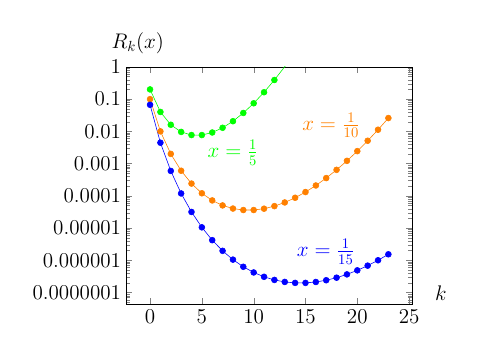
\begin{tikzpicture} [ scale=0.53, every mark/.append style={mark size=2pt} ]
\begin{axis}[
    ymode=log,
    log ticks with fixed point,
    ticklabel style = {font=\Large },
    ymax=1,
    x label style={font=\Large ,at={(axis description cs:1.1,0.1)}},
    y label style={font=\Large ,at={(axis description cs:0.15,1.1)},rotate=270},
    xlabel={$k$},
    ylabel={$R_k(x)$}
    % for log axes, y filter operates on LOGS.
    % and log(y * 1000) = log(y) + log(1000):
    % x filter/.code=\pgfmathparse{#1 + 6.90775527898214
]
\addplot  [
orange, mark=*
]  table {  % 1/10   % Print[Grid[   Table[{k, DecimalForm[N[Factorial[k]*(1/10)^(k + 1)]]}, {k, 0,    23}]]]
 0 0.10000000000000000000
 1 0.010000000000000000000
 2 0.0020000000000000000000
 3 0.00060000000000000000000
 4 0.00024000000000000000000
 5 0.00012000000000000000000
 6 0.000072000000000000000000
 7 0.000050400000000000000000
 8 0.000040320000000000000000
 9 0.000036288000000000000000
 10 0.000036288000000000000000
 11 0.000039916800000000000000
 12 0.000047900160000000000000
 13 0.000062270208000000000000
 14 0.000087178291200000000000
 15 0.00013076743680000000000
 16 0.00020922789888000000000
 17 0.00035568742809600000000
 18 0.00064023737057280000000
 19 0.0012164510040883200000
 20 0.0024329020081766400000
 21 0.0051090942171709440000
 22 0.011240007277776076800
 23 0.025852016738884976640
}
 node [pos=0.9 , above left, style={font=\Large}] {$x=\frac{1}{10}$};


\addplot  [
blue, mark=*
]  table {        % Print[Grid[   Table[{k, DecimalForm[N[Factorial[k]*(1/15)^(k + 1)]]}, {k, 0,    23}]]]
 0       0.0666667
1       0.00444444
2       0.000592593
3       0.000118519
4       0.0000316049
5       0.000010535
6       0.00000421399
7       0.00000196653
8       0.00000104882
9       0.000000629289
10      0.000000419526
11      0.000000307653
12      0.000000246122
13      0.000000213306
14      0.000000199085
15      0.000000199085
16      0.000000212358
17      0.000000240672
18      0.000000288807
19      0.000000365822
20      0.000000487762
21      0.000000682867
22      0.00000100154
23      0.00000153569
}
 node [pos=0.9 , above left, style={font=\Large}] {$x=\frac{1}{15}$};

\addplot  [
green, mark=*
]  table {        % Print[Grid[   Table[{k, DecimalForm[N[Factorial[k]*(1/5)^(k + 1)]]}, {k, 0,    23}]]]
 0       0.2
1       0.04
2       0.016
3       0.0096
4       0.00768
5       0.00768
6       0.009216
7       0.0129024
8       0.0206438
9       0.0371589
10      0.0743178
11      0.163499
12      0.392398
13      1.02024
14      2.85666
15      8.56997
16      27.4239
17      93.2413
18      335.669
19      1275.54
20      5102.17
21      21429.1
22      94288.0
23      433725.0
}
 node [pos=0.2 , below right, style={font=\Large}] {$x=\frac{1}{5}$};
\end{axis}
\end{tikzpicture}
\end{center}
\caption{The absolute error $R_k(x)$ as a function of increasing $k$
for $x\in \{\frac{1}{5},\frac{1}{10},\frac{1}{15}\}$.}
  \label{2018-mm-ferror}
\end{marginfigure}
% ListLogPlot[ Table[Factorial[k]*(1/10)^(k + 1), {k, 0, 23}]]
% Table[{k,N[Factorial[k]*(1/10)^(k + 1),20]}, {k, 0, 23}]
However, this suppression of the absolute error as $k$ grows is eventually
-- that is, if $k > \frac{1}{x}$ -- compensated by the factorial function,
as depicted in Figure~\ref{2018-mm-ferror}: from $k \approx \frac{1}{x}$ the absolute error grows again,
so that the overall behavior of the absolute error $R_k(x)$  as a function of $k$ (at constant $x$)
is ``bathtub''-shaped; with a ``sink'' or minimum at $k \approx \frac{1}{x}$.


\section{Divergence of perturbation series in quantum field theory}

A formal entity such as the solution of an ordinary differential equation may have very
different representations and encodings; some of them with problematic issues.
The means available are often not a matter of choice but of pragmatism and even desperation.\cite{Boyd99thedevil}

This seems to apply also to field theories:
often one is restricted to perturbative solutions in terms of power series.
But these methods are problematic as they are applied in a situation where they are forbidden.

Presently there are two known reasons for the occurrence of asymptotically divergent power series in perturbative quantum field theories:
one is associated with expansion at an essential singularity,  such as $z=0$ for the function $e^\frac{1}{z}$
%https://sites.oxy.edu/ron/math/312/14/ws/24.pdf
and the other with an exchange of the order of two limits,
such as exchanging an infinite sum with an integral if the domain of integration is not compact.

\newpage

\subsection{Expansion at an essential singularity}

The following argument is due to Dyson.\cite{PhysRev.85.631,LeGuillou-Zinn-Justin,Svozil-2023-axioms12010072}
Suppose
the overall energy of a system of a large number $N \gg 1$ of particles
of charge $q$ with mean kinetic energy (aka ``temperature'') $T$
and mean absolute potential $V$
consists of a kinetic and a potential part, like
\begin{equation}
E\sim T N + q^2 V \frac{N(N-1)}{2}\approx T N + \frac{q^2V}{2} N^2,
\label{2019-mm-ch-di-en}
\end{equation}
where ${N(N-1)}/{2}$ is the number of particle pairs.
Then the ground state energy is bound from below as long as the interaction is repulsive: that is, $q^2>0$.
However, for an attractive effective interaction $q^2<0$ and, in particular,
in the presence of (electron-positron) pair creation, the ground state may no longer be stable.
As a result of this instability of the ground state ``around'' $q^2=0$
one must expect that any physical quantity $F(q^2)$ which is calculated as a formal
power series in the coupling constant $q^2$ cannot be analytic around $q^2=0$.
Because, intuitively, even if $F(q^2)$ appears to be ``well behaved'' $F(-q^2)$ is not
if the theory is unstable for transitions from a repulsive to an attractive potential regime.


\marginnote{However, Dyson's argument does not apply to other series solutions~ \bibentry{Watson1912,Weniger2010}
which, for instance, converges on some open half-plane, such as the Dirichlet series.}
Therefore, it is strictly disallowed to develop $F(q^2)$ at $q^2=0$ into a Taylor series.
Insistence (or ignorance) in doing what is forbidden is penalized by an asymptotic divergent series at best.


To obtain a quantitative feeling for what is going on in such cases consider\cite{sommer-AR},
the functional integral
with a redefined exponential kernel from Equation~(\ref{2019-mm-ch-di-en}):
let $N=x^2$,   $T  = -\alpha$, and $g = - \frac{q^2V}{2}$, and
\begin{equation}
f\left(\alpha,g\right)=\int_{0}^{\infty}e^{-\alpha x^{2}-gx^{4}}dx  .
\label{2019-mm-ch-di-en2}
\end{equation}

For negative $g<0$ the term  $e^{-gx^{4}}=e^{|g|x^{4}}$ dominates the kernel, and the integral~(\ref{2019-mm-ch-di-en2}) diverges.
For $\alpha>0$ und $g>0$  this integral has a nonperturbative representation as
\begin{equation}
f\left(\alpha,g\right)=\frac{1}{4}\sqrt{\frac{\alpha}{g}}e^{\frac{\alpha^{2}}{8g}}K_{\frac{1}{4}}\left(\frac{\alpha^{2}}{8g}\right) ,
\label{2019-mm-ch-di-ennp}
\end{equation}
where $K_{\nu}\left(x\right)$ is the modified Bessel funktion of the second kind
(e.g., {\S}9.6, pp.~374-377  of Abramowitz and Stegun).
\marginnote{\url{http://mathworld.wolfram.com/ModifiedBesselFunctionoftheSecondKind.html}}

A divergent series is obtained by expanding $f\left(\alpha,g\right)$ from~(\ref{2019-mm-ch-di-en2})
in a Taylor series of the ``coupling constant'' $g\neq 0$
at $g=0$; and, in particular, by taking the limit $n\rightarrow \infty$ of the partial sum up to order $n$ of $g$:
\begin{equation}
\begin{split}
f_{n}\left(\alpha,g\right)
=
\frac{1}{2}\sum_{k=0}^{n}\frac{\left(-1\right)^{k}}{k!}\frac{\varGamma\left(2k+\frac{1}{2}\right)}{\alpha^{2k+\frac{1}{2}}}g^{k}
\qquad \qquad
\\=
\frac{1}{2}\left[
\sqrt{\pi}
+
\sum_{k=1}^{n}\frac{\left(-1\right)^{k}}{k!}\frac{\varGamma\left(2k+\frac{1}{2}\right)}{\alpha^{2k+\frac{1}{2}}}g^{k}
\right]
\\
=
\frac{1}{2 \sqrt{a}} \left(-\frac{g}{a^2}\right)^n \frac{\Gamma \left(\frac{1}{2} (4 n+1)\right)}{ \Gamma (n+1)}
{\;}_2F_2\left(1,-n;\frac{1}{4}-n,\frac{3}{4}-n;\frac{a^2}{4 g}\right)
.
\label{2019-mm-ch-di-en3}
\end{split}
\end{equation}

% f[a_, g_] = Integrate[E^(-a x^2 - g x^4), {x, 0, Infinity}]

% ff[n_, a_, g_] = (1/2) (Sum[(-g)^k*Gamma[2 k + (1/2)]/(k! a^(2 k + 1/2)), {k, 0, n}])

% ListPlot[Log[N[Abs[Table[ ff[n, 1, 1] - N[f[1, 1]], {n, 1, 10}]]]]]

For fixed $\alpha=1$ the asymptotic divergence of~(\ref{2019-mm-ch-di-en3})
for $n \rightarrow \infty$ manifests itself differently for different values of $g>0$:
\begin{itemize}
\item For $g=1$   the nonperturbative expression~(\ref{2019-mm-ch-di-ennp}) yields
\begin{equation}
f\left(1,1\right)=\int_{0}^{\infty}e^{-x^{2}-x^{4}}dx=\frac{1}{4}  e^\frac{1}{8} K_{\frac{1}{4}}\left(\frac{1}{8}\right)\approx 0.684213  ,
\end{equation}
and
the series~(\ref{2019-mm-ch-di-en3})  starts diverging almost immediately
as the logarithm of the absolute error defined by
$R_n(1)= \log \left| f \left(1,1\right)-f_n \left(1,1\right)\right|$
and depicted in Figure~\ref{2019-mm-ferror1}, diverges.
% fff[n_] = FullSimplify[f[1, 1] - ff[n, 1, 1]]
% Table[N[Log[Abs[fff[n]]]], {n, 0, 20}]
\begin{marginfigure}
{\color{black}
\begin{center}
\begin{tabular}{c}
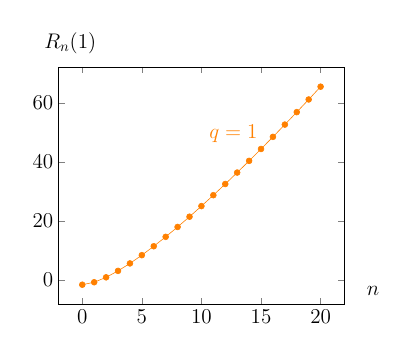
\begin{tikzpicture} [ scale=0.53, every mark/.append style={mark size=2pt} ]
\begin{axis}[
    %ymode=log,
    log ticks with fixed point,
    ticklabel style = {font=\Large },
    %ymax=1,
    x label style={font=\Large ,at={(axis description cs:1.1,0.1)}},
    y label style={font=\Large ,at={(axis description cs:0.15,1.1)},rotate=270},
    xlabel={$n$},
    ylabel={$R_n(1)$}
    % for log axes, y filter operates on LOGS.
    % and log(y * 1000) = log(y) + log(1000):
    % x filter/.code=\pgfmathparse{#1 + 6.90775527898214
]
\addplot  [
orange, mark=*
]  table {
 0      -1.59942
 1      -0.77077
 2      0.894158
 3      3.07015
 4      5.60152
 5      8.40092
 6      11.414
 7      14.6041
 8      17.9452
 9      21.4178
 10     25.0067
 11     28.6999
 12     32.4877
 13     36.362
 14     40.3158
 15     44.3434
 16     48.4397
 17     52.6003
 18     56.8213
 19     61.0993
 20     65.4313
}
 node [pos=0.7 , above left, style={font=\Large}] {$q=1$};

\end{axis}
\end{tikzpicture}
\\
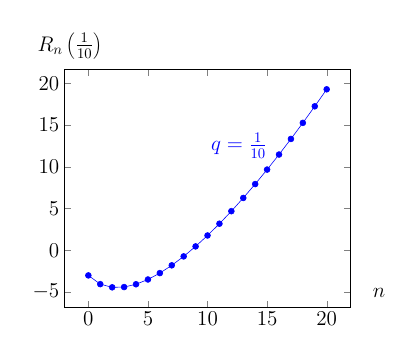
\begin{tikzpicture} [ scale=0.53, every mark/.append style={mark size=2pt} ]
\begin{axis}[
    %ymode=log,
    log ticks with fixed point,
    ticklabel style = {font=\Large },
    %ymax=1,
    x label style={font=\Large ,at={(axis description cs:1.1,0.1)}},
    y label style={font=\Large ,at={(axis description cs:0.15,1.1)},rotate=270},
    xlabel={$n$},
    ylabel={$R_n \left(\frac{1}{10}\right)$}
    % for log axes, y filter operates on LOGS.
    % and log(y * 1000) = log(y) + log(1000):
    % x filter/.code=\pgfmathparse{#1 + 6.90775527898214
]
\addplot  [
blue, mark=*
]  table {
 0   -3.01219
 1   -4.05803
 2   -4.43997
 3   -4.4068
 4   -4.07194
 5   -3.50072
 6   -2.73561
 7   -1.80645
 8   -0.735293
 9   0.460913
 10  1.76876
 11  3.17737
 12  4.67777
 13  6.26244
 14  7.92495
 15  9.65979
 16  11.4622
 17  13.3279
 18  15.2532
 19  17.2348
 20  19.2698
}
 node [pos=0.7 , above left, style={font=\Large}] {$q=\frac{1}{10}$};

\end{axis}
\end{tikzpicture}
\\
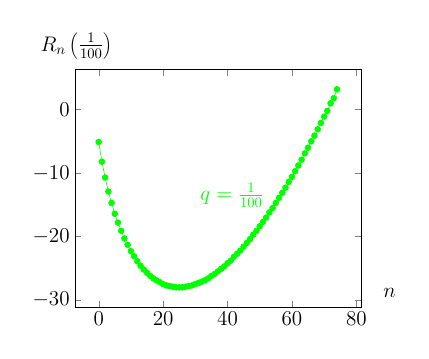
\begin{tikzpicture} [ scale=0.53, every mark/.append style={mark size=2pt} ]
\begin{axis}[
    %ymode=log,
    log ticks with fixed point,
    ticklabel style = {font=\Large },
    %ymax=1,
    x label style={font=\Large ,at={(axis description cs:1.1,0.1)}},
    y label style={font=\Large ,at={(axis description cs:0.15,1.1)},rotate=270},
    xlabel={$n$},
    ylabel={$R_n \left(\frac{1}{100}\right)$}
    % for log axes, y filter operates on LOGS.
    % and log(y * 1000) = log(y) + log(1000):
    % x filter/.code=\pgfmathparse{#1 + 6.90775527898214
]
\addplot  [
green, mark=*
]  table {
 0        -5.1
 1        -8.2
 2        -10.7
 3        -12.9
 4        -14.7
 5        -16.4
 6        -17.8
 7        -19.1
 8        -20.3
 9        -21.3
 10       -22.3
 11       -23.1
 12       -23.9
 13       -24.6
 14       -25.2
 15       -25.7
 16       -26.2
 17       -26.6
 18       -26.9
 19       -27.2
 20       -27.5
 21       -27.7
 22       -27.8
 23       -27.9
 24       -28.0
 25       -28.0
 26       -28.0
 27       -27.9
 28       -27.8
 29       -27.7
 30       -27.5
 31       -27.3
 32       -27.1
 33       -26.9
 34       -26.6
 35       -26.2
 36       -25.9
 37       -25.5
 38       -25.1
 39       -24.7
 40       -24.2
 41       -23.8
 42       -23.2
 43       -22.7
 44       -22.2
 45       -21.6
 46       -21.0
 47       -20.4
 48       -19.7
 49       -19.1
 50       -18.4
 51       -17.7
 52       -17.0
 53       -16.2
 54       -15.5
 55       -14.7
 56       -13.9
 57       -13.1
 58       -12.3
 59       -11.4
 60       -10.6
 61       -9.7
 62       -8.8
 63       -7.9
 64       -6.9
 65       -6.0
 66       -5.0
 67       -4.1
 68       -3.1
 69       -2.1
 70       -1.1
 71       -0.2
 72       1.0
 73       1.8
 74       3.2
}
 node [pos=0.7 , above left, style={font=\Large}] {$q=\frac{1}{100}$};

\end{axis}
\end{tikzpicture}
\end{tabular}
\end{center}
\caption{The logarithm of the absolute error $R_n$ as a function of increasing $n$
for $q\in \{1,\frac{1}{10},\frac{1}{100}\}$, respectively.\label{2019-mm-ferror1}     }
}
\end{marginfigure}

\item For $g=\frac{1}{10}$   the nonperturbative expression~(\ref{2019-mm-ch-di-ennp}) yields
\begin{equation}
f\left(1,\frac{1}{10}\right)=\int_{0}^{\infty}e^{-x^{2}-\frac{1}{10}x^{4}}dx =\frac{1}{2}\sqrt{\frac{5}{2}}e^{\frac{5}{4}}K_{\frac{1}{4}}\left(\frac{5}{4}\right)\approx 0.837043  ,
\end{equation}
and
the series~(\ref{2019-mm-ch-di-en3})  performs best at around $n=3$ or $4$ and then starts to deteriorate
as the logarithm of the absolute error defined by
$R_n \left(\frac{1}{10}\right)=  \log \left| f \left(1,\frac{1}{10}\right)-f_n \left(1,\frac{1}{10}\right)\right| $
and depicted in Figure~\ref{2019-mm-ferror1}, diverges.
%
% ffff[n_] = FullSimplify[f[1, 1/10] - ff[n, 1, 1/10]]
% able[N[Log[Abs[ffff[n]]]], {n, 0, 20}]
%

\item For $g=\frac{1}{100}$ (a value which is almost as small as the coupling constant $g=\frac{1}{137}$ in quantum electrodynamics)
the nonperturbative expression~(\ref{2019-mm-ch-di-ennp}) yields
\begin{equation}
f\left(1,\frac{1}{100}\right)
=\int_{0}^{\infty}e^{-x^{2}-\frac{1}{100}x^{4}}dx
=\frac{5}{2}e^{\frac{25}{2}}K_{\frac{1}{4}}\left(\frac{25}{2}\right)\approx 0.879 849 554 945 695
.
\end{equation}
The series~(\ref{2019-mm-ch-di-en3}) performs best at around $n=25$ and then starts to deteriorate
as the logarithm of the absolute error defined by
$R_n \left(\frac{1}{100}\right) =  \log \left| f \left(1,\frac{1}{100}\right)-f_n \left(1,\frac{1}{100}\right)\right| $
and depicted in Figure~\ref{2019-mm-ferror1}, diverges.
\end{itemize}


\subsection{Forbidden interchange of limits}

A second ``source'' of divergence is the forbidden and thus incorrect interchange of limits --
in particular, an interchange between sums and integrals~\sidenote[][25mm]{See, for instance, the discussion in
Section~II.A of  \bibentry{PhysRevD.57.1144} based on  Lebesgue's dominated convergence theorem.} --
during the construction of the perturbation series.
Again one may perceive asymptotic divergence as a ``penalty'' for such manipulations.
%https://en.wikipedia.org/wiki/Interchange_of_limiting_operations

For the sake of a demonstration, consider again the integral~(\ref{2019-mm-ch-di-en2})
\begin{equation}
f\left(1,g\right)
=\int_{0}^{\infty}e^{- x^{2}-gx^{4}}dx
=\int_{0}^{\infty}e^{- x^{2}}e^{-gx^{4}}dx
\label{2019-mm-ch-di-en3a}
\end{equation}
with $\alpha=1$. A Taylor expansion of the ``interaction part'' in the ``coupling constant'' $g$
of its kernel at $g=0$ yields
\begin{equation}
e^{-gx^{4}} =\sum_{k=0}^\infty \left(-x^4\right)^n \frac{1}{k!} g^k.
\label{2019-mm-ch-di-en3eip}
\end{equation}
This is perfectly legal; no harm done yet.
Consider the resulting kernel as a function of  the order $k$
of the Taylor series expansion, as well as of the ``coupling constant'' $g$
 and of the integration parameter $x$
for $\alpha=1$ in a similar notation as introduced in Equation~(\ref{2019-mm-ch-di-en3}):
\begin{equation}
F_k(g,x)= \frac{\left(-g\right)^k}{k!} e^{- x^{2}} x^{4k} .
\label{2019-mm-ch-di-en3eipke}
\end{equation}
Rather than  applying Lebesgue's dominated convergence theorem to $F_k(g,x)$
we directly show that an interchange of summation with integration yields a divergent series.

%Sum[(-g)^n/(n!) E^(-x^2) x^(4 n), {n, 0, Infinity}]
%E^(-x^2 - g x^4)

Indeed, the original order of limits in~(\ref{2019-mm-ch-di-en2})
yields a convergent expression~(\ref{2019-mm-ch-di-ennp}):
\begin{equation}
\begin{split}
\lim_{t\rightarrow \infty}
\lim_{n\rightarrow \infty}
\int_0^t dx
\sum_{k=0}^n
F_k(g,x) \qquad \qquad \\
=
\int_{0}^{\infty}e^{-x^{2}-gx^{4}}dx  = f\left(1,g\right)=
\frac{1}{4}\sqrt{\frac{1}{g}}e^{\frac{1}{8g}}K_{\frac{1}{4}}\left(\frac{1}{8g}\right)
.
\label{2019-mm-ch-di-en3eipke2c1}
\end{split}
\end{equation}

However, for $g\neq 0$ the interchange of limits results in a divergent series:
\begin{equation}
\begin{split}
\lim_{n\rightarrow \infty}
\lim_{t\rightarrow \infty}
\sum_{i=0}^n
\int_0^t
F_n(1,g,x)   dx =
\lim_{n\rightarrow \infty}
  f_n\left(1,g\right)   \\
=\lim_{n\rightarrow \infty}
\frac{1}{2}
\sum_{i=0}^n
\frac{(-g)^k}{k!} \Gamma\left(2k+\frac{1}{2}\right)
=
\frac{1}{2}\left[
\sqrt{\pi}
+
\lim_{n\rightarrow \infty}\sum_{i=1}^n
\frac{(-g)^k}{k!} \Gamma\left(2k+\frac{1}{2}\right)
\right].
\label{2019-mm-ch-di-en3eipke2c2}
\end{split}
\end{equation}

%with $\lim_{k\rightarrow \infty} \frac{\Gamma\left(2k+\frac{1}{2}\right}{k!}
Notice that both the direct Taylor expansion of $f(\alpha,g)$ at the singular point $z=0$ as well as the
interchange of the summation from the legal Taylor expansion of $e^{-gx^{4}}$ with the integration in~(\ref{2019-mm-ch-di-en3eipke2c1})
yield the same (asymptotic) divergent expressions~(\ref{2019-mm-ch-di-en3})
and~(\ref{2019-mm-ch-di-en3eipke2c2}).


%Sum[(-g)^n/(n!) E^(-x^2) x^(4 n), {n, 0, Infinity}]
%E^(-x^2 - g x^4)

\subsection{On the usefulness of asymptotic expansions in quantum field theory}

It may come as a surprise that calculations involving asymptotic expansions in the coupling constants yield perturbation series
which perform well for many empirical predictions -- in some cases\cite[-30mm]{HAGIWARA2007173}
the differences between experiment and prediction as small as $10^{-9}$.
Depending on the temperament and personal inclinations to accept results from ``wrong'' evaluations
this may be perceived optimistically as well as pessimistically.

As we have seen the quality of such asymptotic expansions depends on the magnitude of the expansion parameter:
the higher it gets the worse is the quality of prediction in larger orders.
And the approximation will never be able to reach absolute accuracy.
However in regimes such as quantum electrodynamics,
for which the expansion parameter is of the order of 100, for all practical purposes\cite[-30mm]{bell-a}
and relative to our limited  means to compute the high order terms,
such an asymptotic divergent perturbative expansion
might be ``good enough'' anyway.
But what if this parameter is of the order of $1$?

Another question is whether resummation procedures can ``recover'' the ``right'' solution in terms of analytic functions.
This is an ongoing field of research. As long as low-dimensional toy models such as
the one covered in earlier sections are studied this might be possible, say, by (variants) of Borel summations.\cite[-45mm]{Sauzin-2014,Mas-2019}
However, for realistic, four-dimensional field theoretic models the situation may be very different and ``much harder.''\cite[-25mm]{ZINNJUSTIN20101454,neumaier-sum}
Let me finally quote Arthur M. Jaffe and Edward Witten:\cite{Jaffe-Witten-2000-QYMT}
{\em ``In most known examples, perturbation series,
i.e., power series in the coupling constant, are divergent expansions; even Borel and
other resummation methods have limited applicability.''}







\begin{center}
{\color{olive}   \Huge
%\decofourright
 %\decofourright
%\decofourleft
%\aldine X \decoone c
 \floweroneright
% \aldineleft ]
% \decosix
%\leafleft
% \aldineright  w  \decothreeleft f \leafNE
% \aldinesmall Z \decothreeright h \leafright
% \decofourleft a \decotwo d \starredbullet
%\decofourright
% \floweroneleft
}
\end{center}

